\documentclass{report}

\usepackage{array} 
\usepackage{comment}
\usepackage{graphicx}
\usepackage[T1]{fontenc}
\usepackage{csquotes}
\usepackage{balance}
\usepackage{setspace}
\usepackage[table]{xcolor}

\usepackage{lstautogobble}
\usepackage{subcaption}

\usepackage{standalone}
\usepackage{algorithmicx}

\usepackage{amsmath}
\usepackage{amssymb}

\usepackage{tikz}
\newcommand\setrow[6]{
  \setcounter{col}{1}
  \foreach \n in {#1, #2, #3, #4, #5, #6} {
    \edef\x{\value{col} - 0.5}
    \edef\y{6.5 - \value{row}}
    \node[anchor=center] at (\x, \y) {\n};
    \stepcounter{col}
  }
  \stepcounter{row}
}
\newcounter{row}
\newcounter{col}

\usepackage{lineno}
\linenumbers

\usepackage[normalem]{ulem}

\usepackage{hyperref}
\hypersetup{hidelinks}

\usepackage{listings}
\lstset{ %
language=C++,                % choose the language of the code
basicstyle=\ttfamily\footnotesize,       % the size of the fonts that are used for the code
commentstyle = \color{ForestGreen},
columns=fullflexible,
numbers=left,                   % where to put the line-numbers
numberstyle=\footnotesize,      % the size of the fonts that are used for the line-numbers
stepnumber=1,                   % the step between two line-numbers. If it is 1 each line will be numbered
numbersep=5pt,                  % how far the line-numbers are from the code
%backgroundcolor=\color{codeBG3},  % choose the background color. You must add \usepackage{color}
showspaces=false,               % show spaces adding particular underscores
showstringspaces=false,         % underline spaces within strings
showtabs=false,                 % show tabs within strings adding particular underscores
frame=single,           % adds a frame around the code
tabsize=2,          % sets default tabsize to 2 spaces
captionpos=b           % sets the caption-position to bottom
breaklines=true,        % sets automatic line breaking
breakatwhitespace=false,    % sets if automatic breaks should only happen at whitespace
keywordstyle=\color{blue},       % keyword style
  %language=Octave,                 % the language of the code
  otherkeywords={SearchVar,MV,TSS,tileExpr,Search,tFunc...},           % if you want to add more keywords to the set
  numberstyle=\tiny\color{black}, % the style that is used for the line-numbers
  rulecolor=\color{black},
escapeinside={<@}{@>}
} 
\definecolor{ForestGreen}{RGB}{34,139,34}
\newcommand{\todo}[1]{{\textcolor{red}{{\tt{TODO:}}\,\,#1 }}}
\newcommand{\nc}[0]{\todo{cite}}
\newcommand{\an}[1]{{\textcolor{blue}{Author's Note: #1}}}
\newcommand{\ttt}[1]{{\texttt{#1}}}
\usepackage{xspace}
\newcommand{\FormatDecisions}[0]{{\textsc{FormatDecisions}}}
\newcommand{\su}[1]{{#1$\times$}}
\graphicspath{{./graphics/}{.}{./graphics/FormatDecisions}{./graphics/RAJALC}}

\usepackage[subtle]{savetrees}
\vbadness=18000

\begin{document}

%\chapter{Introduction}

%\chapter{Schedule Transformations}\label{chap:RAJALC}

Typical parallelization approaches such as OpenMP and CUDA provide constructs for parallelizing and blocking for data locality for individual loops.
By focusing on each loop separately, these approaches fail to leverage sources of data locality possible due to inter-loop data reuse.
The loop chain abstraction provides a framework for reasoning about and applying inter-loop optimizations.
In this chapter, I incorporate the loop chain abstraction into RAJA, a performance portability library for high-performance computing applications.
Using the loop-chain-extended RAJA, or RAJALC, developers can have the RAJA library apply schedule transformations like loop fusion and overlapped tiling while maintaining the original structure of their programs. 
By introducing targeted symbolic evaluation capabilities, RAJALC can collect and cache data access information required to verify loop transformations.
I evaluate the performance improvement and refactoring costs of other extension.
Overall, the results demonstrate 85--98\% of the performance improvements of hand-optimized kernels with dramatically fewer code changes.

\section{Introduction and Summary}
Scientific inquiry leverages high-performance computing (HPC) for a variety of
tasks, including data analysis and experiment design. 
Also, experiments are often performed \textit{in silico}, using 
simulation instead of real-world experiment.
Further, the rise of machine learning gives HPC principles wider
applicability than ever before.

HPC systems are incredibly diverse architecturally, 
both in terms of compute and data.
The ten fastest HPC systems use nine different processor/coprocessor
configurations~\cite{top500}.
This architectural diversity implies that applications designed to be
performant on one system do not necessarily perform well on others.
%Sorta C1
Because the labor costs of developing a new version of an application are so high, 
there is a need for tools that allow developers to design a single application
that performs well across systems with minimal modifications.

Performance portability libraries like RAJA~\cite{hornung2014RAJA} do exactly this.
These libraries enables programmers to specify loops with templated functions,
where one template parameter is an execution policy that describes how a computation should be run.
In RAJA, examples of these policies include \verb.simd_exec. (vectorized), \verb.omp_parallel_for_exec. (OpenMP threading), or \verb.cuda_exec. (GPU).
Thus the heavy lifting of porting a parallel implementation to different 
architectures is abstracted into standardized execution policies.


When optimizing an application, loops are generally considered and
parallelized one at a time.
Optimizing the performance of HPC applications is more complicated than introducing new parallelism.
Many applications are not compute-bound, meaning additional parallelism does not improve performance. 
Instead, moving data to and from memory and accelerators bottlenecks these applications. 
While PPLs support porting per-loop parallelism between systems, they lack the ability to port inter-loop schedule transformations that improve data locality. 
The key capability they need to enable porting these transformations is an inter-loop scope.
The loop chain abstraction provides exactly this.

The loop chain abstraction~\cite{krieger2013loop} captures sequences of loops that share 
data and enough information about how such loops access 
data to enable inter-loop optimization.
Considering loops as a chain uncovers optimizations, like fusion
and overlapped tiling, that are impossible to replicate when optimizing
each loop independently.
\textbf{I address the problem in porting data locality optimizations in this
work by incorporating loop chaining, an abstraction for balancing data locality
with parallelism across loops, into a representative performance portability library, RAJA.}
The technique imposes a minimal code delta on the developer, leverages C++'s
operator overloading and generic lambdas to perform necessary analysis, and
requires no additional compilation steps.

This chapter presents the following contributions:
\begin{itemize}
\item the design of a compact RAJA extension to enable inter-loop
			optimizations;
\item a methodology to perform symbolic evaluation in C++ code;
\item an implementation of these techniques in RAJA\@; and
\item evaluation of their porting costs and performance benefits.
\end{itemize}

For the RAJAPerf case study, RAJALC requires 8.5 source lines of code changed or added on average, compared to 23.625 when implementing by hand.
Furthermore, in 21 of 24 benchmark-system combinations, RAJALC sees performance changes in the same direction as hand-implemented variants, and 85--98\% of the performance improvement, depending on the system.

\section{RAJA's Approach to Portability}

Before making the step to inter-loop representation and optimization, let us the key features of RAJA that enable performance portability
as RAJALC leverages them.
These features are an abstraction layer for data accesses and the
orthogonal specification of loop schedules
(i.e., separating the specification of the loop body from the loop iteration).
Current usage of RAJA leverages these for loop parallelization and
data layout transformations.
In this paper, I use these features to build the loop chain abstraction.

\subsection{RAJA HYDRO\_2D Example}
%First person plural bc its me and the reader walking through stuff
To illustrate the loop and data access abstraction and to provide context
for the required coding effort, I port a loop in the HYDRO\_2D benchmark
from its reference C/C++ implementation to use RAJA\@.
Listing~\ref{hydroPort} shows the before and after for the port.

RAJA has two built-in execution primitives: \verb.forall. and \verb.kernel..
\verb.forall. is used for unnested loops, so for this example we use
\verb.kernel..
We must provide three pieces of information to \verb.kernel.. 
First, we provide the execution policy, which describes the structure of
the loop and what parts to run in parallel.
Second, we provide a container of iterator tuples, which describe the
iterator values for the loop execution.
Last, we provide a lambda function that describes the loop body.


Another useful step employs RAJA's array wrapper, the View, which supports
easily changing the layout of arrays.
Their use is generally optional with RAJA, but is required to use the loop
chain abstraction.
The abstraction requires data access information, which we collect by
overloading View operators.
Lines 10--11 of Listing~\ref{hydroPort} show how to initialize \verb.zrout.
as a View object.

\begin{figure}
\begin{lstlisting}[label={hydroPort},
    caption={Hydro\_2D Loop (Color indicates code regions of original and RAJA versions that perform similar functions)}]
//original loop nest
<@\textcolor{red}{for}@>(<@\textcolor{blue}{Index\_type k = kbeg; k < kend; k++}@>) {
  <@\textcolor{orange}{for}@>(<@\textcolor{violet}{Index\_type j = jbeg; j < jend; j++}@>) {              
    <@\textcolor{ForestGreen}{zrout[k][j] = zr[k][j] + t * zu[k][j];}@>
    <@\textcolor{ForestGreen}{zzout[k][j] = zz[k][j] + t * zv[k][j];}@>
  }
}

//initializing View objects, (one for each array)
<@\textcolor{black}{using VIEW\_TYPE = View<double, Layout<2> >;}@>
<@\textcolor{black}{VIEW\_TYPE zrout(new double [kN * jN], kN, jN);}@>


<@\textcolor{black}{using}@> KPol = KernelPolicy<
  <@\textcolor{red}{statement::For<0, RAJA::loop\_exec,}@>
    <@\textcolor{orange}{statement::For<1, RAJA::loop\_exec,}@>
      <@{\textcolor{ForestGreen}{statement::Lambda<0>}@>
    >
  >
>;

kernel<KPol>(make_tuple(<@\textcolor{blue}{RangeSegment(kbeg, kend)}@>,
                           <@\textcolor{violet}{RangeSegment(jbeg, jend)}@>),
               <@\textcolor{ForestGreen}{[=] (int k, int j) \{}@>
                 <@\textcolor{ForestGreen}{zrout(k,j) = zr(k,j) + t * zu(k,j);}@>
                 <@\textcolor{ForestGreen}{zzout(k,j) = zz(k,j) + t * zv(k,j);}@>
              <@\textcolor{ForestGreen}{ \}}@>);
\end{lstlisting}
\end{figure}

\subsection{Impact of RAJA}

RAJA provides a methodology to improve application portability.
As the high end of high performance computing transitions from traditional
homogeneous core designs into heterogeneous systems, applications 
require a common abstraction to keep up with the variety of platforms
and their associated programming models.
RAJA provides that abstraction for LLNL C++ applications, which are large
(i.e., a hundred thousand to low millions of lines), long lived (i.e., often
20 years or greater), and must both run and perform well on cutting-edge
hardware to accomplish their goals.

RAJA has grown into a library that implements the core constructs and
architecture and model-specific policies, across a myriad of platforms and
backends. RAJA is in production use in eight~\cite{raja-ecp-report} distinct
LLNL applications and libraries, as well as several ECP applications including
SW4~\cite{sw4}, GEOSX~\cite{geosx}, and SUNDIALS~\cite{sundials}.

Results published for three LLNL production codes~\cite{raja-p3hpc} show
performance portability across a variety of architectures.  Comparing a whole
node to a whole node, Ares achieved $13\times$, ALE3D achieved $17\times$ and
Ardra achieved $12\times$ speedups on nodes of the LLNL Sierra system for
meaningful inputs.


\section{Loop Chain Abstraction}\label{sec:loopchain}
RAJA loop execution policies apply to individual loops.
Often two or more loops exhibit producer/consumer data sharing.
The loop chain abstraction~\cite{krieger2013loop} enables scheduling
across such loops to improve temporal data locality. 
The goal is to design RAJA techniques to express and to schedule loop chains.

\subsection{Loop Chains}

A loop chain is a sequence of loop nests $L_{0},L_{1},L_{2},\dots,L_{n}$,
in which each loop nest $L_{i}$ has four associated components:
\begin{itemize}
\item an iteration space $I_{i}$,
\item functions $R_{i}$ and $W_{i}$ that map iteration $i$ to the data 
      elements that it reads and writes;
\item a parallelism policy $p_{i}$ that describes how the loop can be executed; and
\item a loop body $B_{i}$.
\end{itemize} 

The loop chain abstraction expands the possible loop scheduling scope.
Using it to optimize an application consists of three stages:
specifying loop objects; specifying or selecting provably correct loop
transformations; and applying those transformations.

\subsection{Loop Chain Transformations}

Every loop nest has a schedule that describes the order in which the 
iterations should execute.
A lexicographical ordering over integer vectors that represent the
iterations describe this schedule.
Consider the loops in Listing~\ref{scheduleVector}, which sum array
\ttt{a} into \ttt{b} and then store a stencil computation on \ttt{b}
into \ttt{c}.

\begin{figure}[t]
	\begin{lstlisting}[label={scheduleVector},caption={Example Loop Chain}]
	for i = 0 to N:
		for j = 0 to M:
			b[i][j] += a[i][j]                     // B0
	for i = 1 to N-1:
		for j = 1 to M-1:
			c[i][j] = b[i-1][j] + b[i][j] + b[i+1][j] / 3;     // B1
	\end{lstlisting}
	\end{figure}


The set $I_{0}=\{[0,i,0,j,0] \; | \; 0 \leq i < N, 0 \leq j < M\}$ describes
the iterations of the first loop while the set of vectors
$I_{1} = \{[1,i,0,j,0] \; | \; 1 \leq i < N-1, 1 \leq j < M-1\}$ describes
those of the second.
Within each tuple, the first element is the loop index, the second and fourth are the iteration of the loop dimensions, and the third and fifth are the statement index within the loop. 
We can describe the sequential loop schedules as the lexicographical ordering over
$\mathbb{Z}^{5}$.

Legal loop transformations and schedules must respect the data dependences
in the program~\cite{frameworkKP95pub}.
These data dependences can be described as relations over the iterations 
of loops.
The example has dependences from the first statement, $B0$, to the second,
$B1$, due to the writes to \ttt{b} in the first loop and the reads from
\ttt{b} in the second. 
The relations $D_{i-1} = \{[0,i,0,j,0] \to [1,i-1,0,j,0]\}$,
$D_{i} = \{[0,i,0,j,0] \to [1,i,0,j,0]\}$, and
$D_{i+1} = \{[0,i,0,j,0] \to [1,i+1,0,j,0]\}$ describe those dependences. 
The relation induced by the read from \ttt{b[i-1][j]} 
%results in $i+1$
%in the relation because 
is due to the data element written in iteration (i,j) of the
first loop being read by iteration $(i-1,j)$ of the second loop. %, not $(i-1,j)$.
%Write-after-write and write-after-read dependences are formulated similarly.

A legal loop transformation maintains dependence relations. 
That is, a transformation is legal if its application to the dependence
relations remains a subset of the schedule relation.
Consider the fusion transformation on the example loops, which maps the
iteration vectors of the second loop from $[1,i,0,j,0]$ to $[0,i,0,j,1]$. 
Its application to the dependence relation $D_{i-1}$ yields
$\{[0,i,0,j,0] \to [0,i-1,0,j,1]\}$.
Thus, $x > y$ in the schedule for any pair of iterations $(x,y)$ that
$D_{i-1}$ relates, and so the transformation is not legal.

The loop chain abstraction uses the information associated with each loop 
nest to build these representations.
The iteration spaces $I_{i}$ and loop bodies $B_{i}$ describe the iteration
vectors; the data access functions $R_{i}$ and $W_{i}$ construct the
dependence relations; and the parallelism policies $p_{i}$ inform the
schedule relations.


\subsection{Loop Objects in RAJA}

Although RAJA does not intrinsically provide chainable loop objects, it has many
of the necessary components.
The execution primitive and common case, \ttt{kernel} and  \ttt{forall}, form
the initial basis for the description of loop nests.
The first kernel argument is a collection of iterator tuples, an explicit
instance of an iteration space.
The parallelism policy is found in the kernel policy template argument.
The loop body is a variable-length list of lambda functions.
This leaves only two data access functions, which are implicitly encoded
within the loop body.
Section~\ref{subsec:accesses} describes the symbolic evaluation extension
that extracts them.

\section{Design Changes to RAJA}

First, I introduce an interface in RAJA for users to specify loop chains and transformations
so as to enable inter-loop optimizations without additional tooling or compilation steps.
Second, I design a symbolic evaluation mechanism that gathers data access patterns of
kernels.
Third, I use this mechanism to analyze kernels at runtime and use the results to automate the generation of a safe execution schedule for the kernels.


Traditional polyhedral optimization techniques are normally broken up into identifying code regions to optimize, converting to a polyhedral representation, analyzing the structure, applying transformations, and generating code.
Because RAJALC operates at the language level rather than the compiler level, my approach is slightly different. While identifying code regions, converting to a polyhedral representation, and analysis are roughly equivalent to compiler-level approaches, transformation and code generation are formulated differently. 
The fundamental difference is that transformation and code generation happen \textit{before} any analysis.

\subsection{RAJA Computations as Objects}
\begin{figure}[t]
	\begin{lstlisting}[caption={Using the \texttt{fuse} and \texttt{overlapped\_tile} transformations.}, label={transformExample}]
	auto lambda1 = [=](auto i) {c(i) = a(i) * b(i);};
	auto lambda2 = [=](auto i) {d(i) = d(i) + c(i);};
	
	auto loop1 = make_forall<simd_exec>(RangeSegment(0,N), lambda1);
	auto loop2 = make_forall<simd_exec>(RangeSegment(0,N), lambda2);
	
	auto fused = fuse(loop1, loop2);
	fused();
	
	
	auto lambda3 = [=](auto i) {b(i) = (a(i-1) + a(i) + a(i+1) ) / 3;};
	auto lambda4 = [=](auto i) {c(i) = (b(i-1) + b(i) + b(i+1) ) / 3;};
	
	auto loop3 = make_forall<...>(RangeSegment(1,N-1), lambda3);
	auto loop4 = make_forall<...>(RangeSegment(1,N-1), lambda4);
	
	//default tile size
	auto tiled_default = overlapped_tile(loop3, loop4);
	//tile size = 64
	auto tiled_64 = overlapped_tile<64>(loop3, loop4);
	tiled_64();
	 \end{lstlisting}
	\end{figure}
Delayed execution is a key design pattern in %optimizing languages like
embedded domain-specific languages such as
Halide~\cite{ragan-kelley2013halide} and Tensorflow~\cite{tensorflow}.
These languages separate the statements that specify a computation from
those that execute it.
In between, the programmer can specify how to schedule and optimize the computation.
However, in standard RAJA, computational \verb.kernel. statements immediately execute the specified computation.
So, I introduce a wrapper class (\verb.KernelWrapper.) that enables execution
to be delayed until after analysis and transformation.
I introduce two functions based on existing kernel execution functions to
create \verb.KernelWrapper.s: \verb.make_forall. and \verb.make_kernel..
They have the same interface as their corresponding execution functions, but
return a \verb.KernelWrapper. object that can be executed or optimized.
Listing~\ref{transformExample} shows these wrapping functions in use. 


\subsection{Gathering Access Information}\label{subsec:accesses}
\begin{figure}[t]
\begin{lstlisting}[label={symExecChanges}, caption={Kernel Lambda Conversion}]
auto original_lambda = [=](idx_t i, idx_t j) {
	a[i][j] += b[i][j];
};

auto converted_lambda = [=](auto i, auto j) { //idx_t -> auto
	a(i,j) += b(i,j); // array -> View
};
\end{lstlisting}
\end{figure}

\begin{figure}
\includegraphics[width=\linewidth]{SymExecProcess.png}
\caption{Symbolic evaluation of a kernel lambda. 
Indexing expressions are evaluated first, then accesses, then statements in terms of accesses.
As assignments are evaluated, the accesses are marked as reads or writes.
Accesses are tracked using the access collector.}\label{symExec}
\end{figure}
Specifying parallelism within RAJA and other programming models can
build on commonly used abstractions such as \verb.forall..
However, determining when inter-loop scheduling transformations such as
loop fusion are legal requires an analysis of the dependences between those loops.
%Data access information is the largest missing piece for enabling loop chains
%in RAJA.
Other loop chain approaches require specification of data access patterns by
hand, which effectively rewrites the loop~\cite{bertolacci2019using}.
The symbolic evaluation mechanism eliminates this effort for the
developer by leveraging RAJA's array wrapping View abstraction.

%We leverage RAJA's array wrapping Views, which use the call operator to access
%arrays.
Using RAJA \verb.Views.,
an array access like \verb.a[i][j][k]. becomes the \verb.View. access \verb.a(i,j,k). as
Listing~\ref{symExecChanges} shows.
I overload the View function call operator with a symbolic iterator type to automate
data access pattern collection through symbolic execution.
%\todo{Brandon, by View call operator do you mean the overloaded parentheses?  Is that the terminology?} 
% yes: https://en.cppreference.com/w/cpp/language/operators#Function_call_operator
To use symbolic evaluation, kernel lambda arguments must be changed to
\verb.auto., which allows normal execution of lambda using index values while
its symbolical evaluation uses symbolic iterators.

Figure~\ref{symExec} shows the process of symbolically evaluating the body of a lambda. 
I break kernel symbolic evaluation into two contexts: indexing and accessing. 
Indexing encompasses the representation and storage of index expressions, like
\verb.i+1. in \verb.a(i+1)..
The symbolic evaluation must retain the entire structure of the index expression 
because the loop's
data access pattern must reflect the difference between \verb.a(i+1). and
\verb.a(i-1)..
Indexing evaluation is shown in steps 2 and 3 of Figure~\ref{symExec}.
Accessing encompasses the statement-level data access semantics of the kernels.
Unlike with indexing, only whether accesses are reads or writes matters,
not the entire structure of the statements.
For example, the analysis needs to know that the statement \verb.c(i) = a(i) + b(i).
reads \verb.a(i). and \verb.b(i). and writes \verb.c(i)., but not that it
adds \verb.a(i). and \verb.b(i)..
Access evaluation is shown in steps 4, 5, and 6 of Figure~\ref{symExec}.
Listing~\ref{ExpressionGrammar} shows the grammar for supported indexing expressions and access statements. 
Behavior for kernels that do not use this grammar is undefined.

Normal RAJA kernel execution only affects the states of its Views. 
However, symbolic evaluation should not change View states. 
Instead, it should only preserve the access information.
I achieve this by adding a class-wide access collector to the symbolic iterator. 
When symbolic accesses are evaluated, they are added to the collector, and updated as reads or writes when assignments are evaluated.
This access collector and its contents at steps 5 and 7 are shown to the right in Figure~\ref{symExec}, and the change can be seen between steps 5 and 6.


\begin{figure}[t]
\begin{lstlisting}[label={ExpressionGrammar},caption={EBNF Grammar to Support Symbolic Evaluation}]
start : Access Assignment Expression
Expression : Expression Operator Operand | Operand
Operand : Access | Int | Double | Iterator
Operator : + | - | * | / | %
Assignment : = | Update
Update: += | -= | *= | /= | %=

Access : Id '(' IndexExpressions ')'
IndexExpressions : IndexExpression | IndexExpression ',' IndexExpressions
IndexExpression : IndexOperand Operator IndexExpression | IndexOperand
IndexOperand : Int | Double | Iterator
\end{lstlisting}
\end{figure}
	
\subsection{Loop Chain Transformation Specifications}\label{sec:transspec}

With computation objects and their access patterns in hand, transformations can finally be applied.
RAJALC supports two transformations, loop fusion and overlapped tiling, each with two variants.
For all transformations, the user provides the target kernel
objects as arguments.
Listing~\ref{transformExample} shows two of these transformations in use.

Fusion transformations combine execution of iterations with the same iterator
values to improve data locality.
They work best for loops with producer-consumer relationships or those that
access the same data.
RAJALC's fusion transformations, \verb.fuse. and \verb.fuse_always., support
a tradeoff between safety and porting cost.
he former uses symbolic execution to determine if the transformation is legal.
The latter applies it prescriptively.
If the user knows the dependences between loops do not impede fusion,
it allows them to fuse kernels that do not use Views. 
On the other hand, \verb.fuse. requires the user to use Views instead
of arrays to limit the fusion transformation to when it is safe.

Overlapped tiling transformations improve data locality
and enables parallelism by performing some redundant computation 
on the surface of the tiles.
They work best for loops with stencil-like access patterns,
where fusion results in a more restricted wavefront parallelism.
RAJALC's two overlapped tiling transformations, \verb.overlapped_tile. and
\verb.overlapped_tile_fuse., differ in the execution schedule within each tile
as Figures~\ref{tileNofuse} and~\ref{tileFuse} show.
Specifically, the schedule within the tile of \verb.overlapped_tile. mimics
a sequential schedule by executing all iterations of the first kernel before
it executes all iterations of the second while \verb.overlapped_tile_fuse.
fuses individual iterations of the loops within each tile.
Lines 11 through 21 of Listing~\ref{transformExample} show how to use these transformations.

When using the \verb.fuse. variant or either overlapped tiling transformation, if analysis shows the transformation to be unsafe, a warning message is printed and the original schedule is used. 

\subsection{Compile- and Run-time Actions}

When the programmer uses a RAJALC loop transformation, the compiler instantiates two different executor types for the entire loop chain. 
The first executor uses the transformed schedule, while the second uses the original schedule. 
Both executors are included with the object returned by the transformation call.

At run-time, when each kernel is initialized, its data access patterns are collected and cached. 
This reduces the cost of the symbolic evaluation by only performing it once, even through kernels are typically executed many times.
Then, the access information is used by the transformation functions to select which schedule should be used.


\begin{figure*}
	\centering

	\begin{subfigure}[t]{0.45\textwidth}
		\centering
		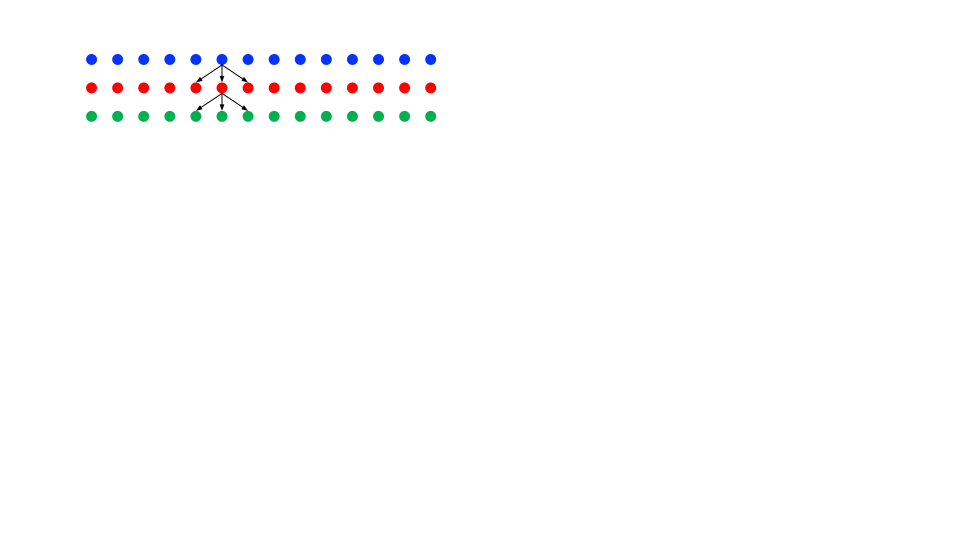
\includegraphics[height=0.45in]{TilingProcess/TilingProcess1.png}
		\caption{Original kernel iteration spaces and abbreviated dependences between iterations.}\label{tiling1}
	\end{subfigure}
	~
	\begin{subfigure}[t]{0.45\textwidth}
		\centering
		\includegraphics[height=.45in]{TilingProcess/TilingProcess2.png}
		\caption{After shifting kernels to remove negative dependences.}\label{tiling2}
	\end{subfigure}
	\par\bigskip
	\begin{subfigure}[t]{0.45\textwidth}
		\centering
\includegraphics[height=0.45in]{TilingProcess/TilingProcess3.png}
		\caption{Shared iteration space. Chain could be fused sequentially.}\label{tiling3}
	\end{subfigure}
	~
	\begin{subfigure}[t]{0.45\textwidth}
		\centering
		\includegraphics[height=.45in]{TilingProcess/TilingProcess4.png}
		\caption{Underlying tiles for TileSize=6 shaded in purple.}\label{tiling4}
	\end{subfigure}
	\par\bigskip
	\begin{subfigure}[t]{0.45\textwidth}
		\centering
		\includegraphics[height=0.45in]{TilingProcess/TilingProcess5.png}
		\caption{Overlap for each tile shaded in orange. Tiles against low edge have no overlap.}
	\end{subfigure}
	~
	\begin{subfigure}[t]{0.45\textwidth}
		\centering
		\includegraphics[height=.45in]{TilingProcess/TilingProcess6.png}
		\caption{An individual overlapped tile.}
	\end{subfigure}
	\par\bigskip
	\begin{subfigure}[t]{0.45\textwidth}
		\centering
		\includegraphics[height=0.45in]{TilingProcess/TilingProcess7.pdf}
		\caption{Execution order for an individual tile without fusion.}\label{tileNofuse}
	\end{subfigure}
	~
	\begin{subfigure}[t]{0.45\textwidth}
		\centering
		\includegraphics[height=0.45in]{TilingProcess/TilingProcess8.pdf}
		\caption{Execution order for an individual tile with fusion.}\label{tileFuse}
	\end{subfigure}
	\par\bigskip
	\begin{subfigure}[t]{\textwidth}
		\centering
		\includegraphics[height=0.45in]{TilingProcess/TilingProcess9.pdf}
		\caption{Global execution order for entire computation.}\label{tiling9}
	\end{subfigure}

\caption{Overlapped tiling of 3 one-dimensional loops.}\label{tilingProcess}
\end{figure*}

\section{Transformations Safety in RAJALC}
Section~\ref{sec:transspec} shows how a user can specify the use of loop fusion transformations
or overlapped and fusion transformations on loops in a chain.
In this section, I describe 
how RAJALC generates different execution schedules and uses the information gathered from the symbolic evaluation to verify their correctness.

\subsection{Loop Shifting for Stencil Computations}

While \verb.fuse_always. prescriptively apples a fusion transformation
without checking its legality, \verb.fuse. uses symbolic evaluation to
guide a legal loop fusion.
For a fusion to be legal, the inter-loop dependences cannot have a
negative direction.
However, loops can often be shifted to make such
dependences non-negative.
Figures~\ref{tiling1} and~\ref{tiling2} show an example of shifting the
loops to adjust negative dependences.
Prior work showed how to convert the dependence relations into constraints
of an ILP optimization problem~\cite{bertolacci2019using}.
RAJALC minimizes the sum of the non-negative shift amounts
$S_{1,1},S_{1,2},\ldots,S_{2,1},\ldots,S_{l,n}$ with the constraints $S_{b,i} + d_i \geq S_{a,i}$ for each dependence
$[d_1,d_2,\ldots,d_n]$ from kernel $a$ to $b$.
Solutions to this problem correspond to shift amounts that enable loop fusion.
RAJALC also use this shifting mechanism to simplify the dependences for overlapped
tiling.

While fusion in this circumstance improves data locality, it restricts
parallelism.
Because fusion combines iterations of different loops, dependences that
are originally between different loops become dependences between iterations
of the same loop. 
While wavefront parallelism may still be possible, overlapped tiling often
offers a better balance of parallelism and data locality~\cite{CathieSC14}.

\subsection{Iteration Space Alignment and Lambda Generation}
When performing optimizing transformations, kernel iteration spaces do not
always completely align. 
Misalignments can arise from differences in the original iteration spaces
or from shifts to remove negative dependences. 
While the iterations the loops in a chain have in common are executed by
the fused or tiled kernels, we also must generate extra kernels to execute
the unshared boundary iterations.

Figure~\ref{fusionPartition} illustrates the generation of these kernels
for one $d=3$ loop in a chain. 
First, RAJALC calculates the shared iteration space of the chain, using the
intersection of all kernel iteration spaces, which yields a $d$-dimensional
hyper-rectangle within each kernel's iteration space, as
Figure~\ref{sharedSpace} shows.
To account for the boundary iterations, RAJALC then partitions the loop's
iteration space, using the faces of the shared iteration space.
Figures~\ref{preshare} and~\ref{postshare} show the iteration spaces of the
$2*d=6$ boundary kernels for the 3D loop. 
This process generates $2*d*n$ boundary kernels across the $n$ loops in a
chain, plus the one fused/tiled kernel over the shared iteration space. 
RAJALC orders these $2*d*n+1$ kernels by loop and dimension to execute the low
boundary iterations, the shared iterations, then the high boundary iterations.

Each kernel requires an iteration space and a lambda describing the loop body. 
For the boundary iterations, RAJALC uses the original lambdas. 
For the shared iterations, a new lambda is generated based on the transformation. 
With fusion, the new lambda executes the sequence of original lambdas, performing one iteration of each loop.
With overlapped tiling, the new lambda executes each original lambda across its share of the tile, as shown in Figure~\ref{tileNofuse}.


\begin{figure}
	\captionsetup[subfigure]{justification=centering}
		\centering
		\begin{subfigure}[t]{0.33\textwidth}
			\centering
			\includegraphics[height=0.5in]{FusionPartition/axes.png}
			\caption{Dimension order of loop.}
		\end{subfigure}
		
	%	\begin{subfigure}[t]{0.33\textwidth}
	%		\centering
	%		\includegraphics[height=1.5in, clip=true, trim=200 0 200 200]{FusionPartition/FusionPartition1.pdf}
	%		\caption{Original iteration space of one loop in chain.}
	%	\end{subfigure}
		
		\begin{subfigure}[t]{0.45\textwidth}
			\centering
			\includegraphics[height=1.5in, clip=true, trim=200 20 200 200]{FusionPartition/FusionPartition2.pdf}
			\caption{Original iteration space of one \\ loop in chain and shared iteration \\ space executed by fused kernel.}\label{sharedSpace}
		\end{subfigure}
		\begin{subfigure}[t]{0.45\textwidth}
			\centering
			\includegraphics[height=1.5in, clip=true, trim=200 20 200 200]{FusionPartition/FusionPartition5.pdf}
			\caption{Lower boundary iteration spaces.}\label{preshare}
		\end{subfigure}
	
		\begin{subfigure}[t]{0.5\textwidth}
			\centering
			\includegraphics[height=1.5in, clip=true, trim=200 20 200 200]{FusionPartition/FusionPartition8.pdf}
			\caption{Higher boundary iteration spaces.}\label{postshare}
		\end{subfigure}
	\caption{Partitioning the iteration space of a single 3d loop. The original iteration space is $(0,10)\times(0,10)\times(0,10)$ and the fused iteration space is $(1,9)\times(2,8)\times(1,8)$. This partitioning process occurs for each kernel in the chain.}\label{fusionPartition}
	\end{figure}
	


\subsection{Overlapped Tiling}

Overlapped tiling proceeds similarly to the \verb.fuse. transformation. 
First, RAJALC calculates and applies shifts to remove negative dependences as
Figures~\ref{tiling1} and~\ref{tiling2} show.
Next, it calculates the overlapping iteration space and partition boundary
iterations as Figure~\ref{tiling3} shows.
Finally, it perform overlapped tiling as Figures~\ref{tiling4}-\ref{tiling9} show.

Before RAJALC can generate the kernel for the overlapped tiling, it must
calculate the overlap amounts. 
This is set up as an ILP optimization problem similarly to the calculation of the
shift amounts.
For $n$ kernels of dimension $m$, the optimization problem is over the $nm$
overlap amounts $O_{1,1},O_{1,2},\ldots,O_{2,1},\ldots,O_{n,m}$.
I introduce a non-negativity constraint to ensure that all overlap amounts
are greater than zero. 
I then add the constraints
$O_{a,1} >= O_{b,1} + d_{1}, O_{a,2} >= O_{b,2} + d_{2},\ldots,O_{a,m} >= O_{b,m} + d_{m}$
for each dependence $D=[d_{1},d_{2},\ldots,d_{m}]$ from kernel $a$ to kernel $b$,
which ensures that if a tile includes an iteration of kernel $b$, it also
includes all necessary iterations of kernel $a$.
Finally, it minimizes the sum of the overlap amounts
$\sum_{i=1}^{n} \sum_{j=1}^{m} O_{i,j}$.

After RAJALC calculates the overlap amounts, it generates a kernel that iterates
over each tile, executing the original kernels for the iterations of the tile.
The two overlapped tiling transformations, \verb.overlapped_tile_no_fuse.
and \verb.overlapped_tile_fuse. differ in their schedule for executing each
tile.
Without fusion, it executes the tile one kernel at a time: all of $knl1$ is
executed, then all of $knl2$, and so on. 
tile sizes are constrained for this schedule by cache size and by the size of
the overlap. 
Tiles must be small enough to fit into cache to maximize data locality
benefits, but tile size should be maximized to reduce the proportion of
recomputation.

In contrast, the \verb.overlapped_tile_fuse. transformation fuses iterations
within each tile using the fusion algorithm described above.
Introducing fusion into the tile decouples data locality from cache size.
Unrestricted by cache considerations, the only limit on tile size is the
need for parallelism, enabling larger tiles than otherwise possible.

\section{Case Study: RAJA Performance Suite}

I evaluate the advances through two case studies, porting the RAJA
Performance Suite (RAJAPerf)~\cite{hornung2017raja} and LULESH from
standard RAJA to RAJALC\@
In both case studies, I evaluate the performance and porting process
of the RAJALC implementations and I detail benefits and limitations
of the approach.

The RAJA Performance Suite is a collection of benchmark kernels that are
used to evaluate RAJA performance.
The suite contains 46 benchmark kernels across five categories; 33 contain
a single loop nest, leaving 13 kernels for which the advances are relevant.
Four of these are matrix computations involving reductions to which 
RAJALC's current capabilities do not apply. 
Finally, one benchmark does not exhibit any data reuse, so no data locality 
optimizations are relevant, including those supported here. 
Thus, I evaluate RAJALC on 8 benchmark kernels.

For each of the 8 kernels, I identify a locality-improving transformation
and implement new variants.
The first variant, \verb.Hand_Opt., applies the transformations directly.
The second variant, \verb.LoopChain., applies the transformation using RAJALC\@.
I record the number of modified or added source lines of code for each
variant and evaluate their performance on three systems.
%Rose
System Intel1 has an 8-core Intel Core i7--6900K CPU at 3.2 GHz and 32G of memory.
% 512K L1 cache, 2M L2 cache, and 20M L3 cache.
It runs Ubuntu 16.04.7 and GCC11.0.
%Quartz
System Intel2 has a 36-core Intel Xeon E5--2695 CPU at 2.1 GHz and 128 GB of memory.
%Lassen
System Power9 has an 44-core IBM Power9 at 3.5 GHz and 256 GB of memory.
Systems Intel2 and Power9 run TOSS 3 and GCC8.3.1.


\subsection{Benchmark Descriptions}

I categorize each benchmark as either point-wise or stencil. 
Point-wise loops access at most one element of each array per iteration,
while stencil loops access a fixed pattern of elements of each array per
iteration. 
The loop bodies
\verb.lambda1. and \verb.lambda2. in Listing~\ref{transformExample} are
examples of point-wise loops, while \verb.lambda3. and \verb.lambda4. are
examples of stencil loops.

Three of the benchmarks, \verb.GEN_LIN_RECUR., \verb.ENERGY., and
\verb.PRESSURE., are point-wise computations.
\verb.GEN_LIN_RECUR. comes from a general linear recurrence computation and
\verb.ENERGY. and \verb.PRESSURE. are loops extracted from LULESH, a
hydrodynamics code. 
For these benchmarks, loop fusion does not interfere with parallelism, so
I apply that transformation.

The other five benchmarks are stencil computations: \verb.JACOBI_1D.,
\verb.JACOBI_2D., \verb.HEAT_3D., \verb.HYDRO_2D., and \verb.FDTD_2D..
\verb.JACOBI_1D., \verb.JACOBI_2D., and \verb.HEAT_3D. compute solutions
to discretized PDEs in their respective dimensions.
\verb.HYDRO_2D. is part of a hydrodynamics code.
\verb.FDTD_2D. is a finite-difference time-domain kernel that is unique
among the stencil computations because I can fuse two of its four loops 
without inhibiting parallelism.
Thus, I apply that transformation.
The other four require shifting to be fused, so I apply overlapped tiling
to retain sufficient parallelism.

\subsection{Porting}

Implementing the fusion transformation is fairly easy. 
For the RAJALC variant, because I can confirm their point-wise nature
visually, symbolic evaluation is unnecessary.
Thus, I directly apply the transformation without converting the kernels to 
RAJA Views.
The hand-applied variant code changes are also low impact; in a real
application they would not be desirable as the kernels may be used separately
in other contexts.
Instead of multiple calls to \verb.RAJA::kernel. with the different loop
bodies, a single call is made with all loop bodies as one.
For the \verb.GEN_LIN_RECUR. benchmark, I also apply a loop reversal
transformation by hand to both variants. RAJALC does not currently support 
loop reversal, but its inclusion in the implementation would not be difficult.
However, automation of its use and its limited applicability in 
existing RAJA applications has made its implementation low priority. 

For \verb.HYDRO_2D., applying overlapped tiling transformation with RAJALC 
requires minimal changes: I add two lines of code and change three. 
In contrast, the hand implementation changes four lines and added 41
new lines, effectively an order of magnitude more effort. 
These additional lines calculate the amounts to shift and to overlap, 
create the new, tiled kernel, and execute the boundary iterations not
within the tiled area. 
These changes are not simple; the porting process encountered errors
in nearly all parts: shifting, boundary iterations, tile sizes, tile
bounds, and tile execution.

Porting effort in source lines of code
for the other three overlapped tiling kernels is similar to 
\verb.HYDRO_2D., with one major difference.  
While \verb.HYDRO_2D. has distinct input and output arrays; \verb.JACOBI_1D., 
\verb.JACOBI_2D., and \verb.HEAT_3D. each use one of two arrays for
input and output, which introduces anti-dependences that inhibit 
overlapped tiling. 
To mitigate this effect, I modify the kernels to use
a double-buffer strategy that eliminates the anti-dependence. 
Listing~\ref{jacobiDoubleBuffer} shows the double-buffer reference
implementation for \verb.JACOBI_1D..
%%
I add the double-buffer transformation by hand in these three variants;
its automation is future work.
I plan to use the access information collected during symbolic evaluation
to identify chains that require it and to implement the double buffer within
the View class.
\begin{figure}[t]
\begin{lstlisting}[label={jacobiDoubleBuffer},caption={Double-Buffer Implementation for JACOBI\_1D}]
for(int t = 0; t < numIters; t++) {
	temp = A1.data_ptr;
	A1.data_ptr = A2.data_ptr;
	A2.data_ptr = temp;
	for(int i = 0; i < length; i++) {
		B(i) = 0.33333 * (A1(i-1) + A1(i) + A1(i+1));
	}
	for(int i = 0; i < length; i++) {
		A2(i) = 0.33333 * (B(i-1) + B(i) + B(i+1));
	}
}
\end{lstlisting}
\end{figure}

Table~\ref{sloc} shows the number of changed and added source lines of code
for all benchmarks.
Overall, manual porting difficulty in source lines of code 
increases as the dimensionality of a 
kernel increases, mostly due to the specification of the boundary iterations. 
Alternatively, RAJALC porting difficulty is similar regardless of the loop
dimensionality.
Also, while with RAJALC code retains its original structure, the 
hand-implemented transformations obscure the underlying computation,
which significantly complicates code maintenance.
\begin{table}[t]
\begin{tabular}{|l|l|l|l|l|}
\hline
\textbf{Benchmark}       & \multicolumn{2}{l|}{\textbf{\begin{tabular}[c]{@{}l@{}}Manual \\ Implementation\end{tabular}}} & \multicolumn{2}{l|}{\textbf{\begin{tabular}[c]{@{}l@{}}RAJALC\\ Implementation\end{tabular}}} \\ \hline
\cellcolor[HTML]{9B9B9B} & Changed                                         & Added                                        & Changed                                        & Added                                        \\ \hline
\textit{ENERGY}          & 6                                               & 6                                            & 6                                              & 2                                            \\
\textit{PRESSURE}        & 2                                               & 3                                            & 2                                              & 2                                            \\
\textit{GEN\_LIN\_RECUR} & 1                                               & 1                                            & 2                                              & 2                                            \\
\textit{FDTD\_2D}        & 8                                               & 4                                            & 9                                              & 4                                            \\
\textit{HYDRO\_2D}       & 4                                               & 41                                           & 3                                              & 2                                            \\
\textit{JACOBI\_1D}      & 3                                               & 17                                           & 3                                              & 3                                            \\
\textit{JACOBI\_2D}      & 10                                              & 33                                           & 10                                             & 3                                            
\\
\textit{HEAT\_3D}        & 12                                              & 38                                           & 12                                             & 3                                            \\ \hline
\textit{Average}        & 5.8                                              & 17.9                                           & 5.9                                            & 2.6                                            \\ \hline
%\textit{Average}        & 5.75                                              & 17.875                                           & 5.875                                            & 2.625                                            \\ \hline
\end{tabular}
\caption{Lines of Code Impact (Excludes double-buffer transformation changes)}\label{sloc}
\end{table}

\subsection{Performance}
\begin{figure}
\includegraphics[width=\linewidth]{results/RajaPerf/Rose/RAJAPerf.png}
\caption{Performance changes of RAJAPerf benchmarks on System Intel1 (higher is better).}\label{RAJAPerfPerf}
\end{figure}
Figure~\ref{RAJAPerfPerf} shows the performance of the hand-implemented
and RAJALC variants relative to the original implementations on System Intel1. 
For the double-buffer implementations, I show the performance relative to an 
un-transformed double-buffer implementation. 
I report the average of ten runs. 

For the fused benchmarks, \verb.GEN_LIN_RECUR. and \verb.FDTD_2D. improve
modestly while \verb.PRESSURE. performance drops slightly, likely due to low amounts of data reuse. 
\verb.ENERGY. runs more than two times faster than the original, likely due
to the larger number of fused kernels than the other benchmarks. 
For all four, the RAJALC variant's performance is comparable to the
hand-implemented loop fusion. 
 
For the overlapped tiled benchmarks, the \verb.Hand_Opt. variant improves
performance up to 22\% for all benchmarks.
The RAJALC variant, which achieves its best performance with different tile sizes, improves performance by 
up to 20\%.
For both variants, the tile sizes were tuned manually.
Overall, the RAJALC variant achieves 85\% of the geometric mean performance
improvement of the hand-implemented variant. 


Because of the large thread counts on Systems Intel2 and Power9, I evaluated the scaling performance of RAJAPerf when using RAJALC\@.
Unlike on System Intel1, RAJAPerf often did not benefit from the inter-loop
optimizations on Systems Intel2 and Power9, even when applied by hand. 
However, the direction of RAJALC's performance impact was nearly identical to the hand-optimized code. 
On System Intel2, 47 of the 48 benchmark-thread-count combinations had the same direction of impact.
On System Power9, all 48 combinations matched the direction of performance impact between the two variants.
Overall, the geometric mean of the fraction of the hand-implemented speedup achieved by RAJALC ranges across thread counts from 0.92 and 0.97 on System Intel2 and 0.95 and 1.02 on System Power9. 
This is evidence that RAJALC is a useful tool for quickly prototyping transformations without large refactoring costs and accurately recreates the performance impact of hand implementing the transformations.

\section{Case Study: LULESH}

While the RAJAPerf case study demonstrates the types of computations RAJALC
can optimize, the second case study, LULESH, explores its potential within a
larger application.
LULESH is a DOE proxy application for shock hydrodynamics codes.
It solves a simple Sedov blast problem using the typical numerical algorithms and computational characteristics for larger codes.

As with the previous case study, I characterize the porting process and
evaluate RAJALC performance compared to the original implementation.
For this evaluation, I ported LULESH v2.0~\cite{LULESH2}. 

\subsection{Porting}

Porting LULESH is more involved than the RAJAPerf kernels. 
I must first identify the part of the application to optimize,.
I choose the function \verb.EvalEOSForElems., which has a long series
of point-wise computations over the same iteration space.
The \verb.ENERGY. and \verb.PRESSURE. benchmarks within RAJAPerf are
from this part of LULESH\@.

\subsubsection{Code Change: Arrays to Views}

The RAJA implementation of LULESH uses RAJA execution statements, but
does not use RAJA Views for arrays and vectors. 
Thus, I first convert these data structures to use Views.
For many of the data structures, array accesses are abstracted through
indexing functions. 
I replace these indexing functions directly with Views without changing
the source code of the algorithms.
However, the existing version often uses arrays, especially for local and
temporary storage.
I wrap these arrays with Views and change the accesses from brackets to
parentheses, a tedious but simple code change.

\subsubsection{Code Change: Kernel Objects}

The second required change uses RAJALC kernel objects instead of direct
code execution.
I move the series of point-wise computations in \verb.EvalEOSForElems. that operate over the same iteration space into many individual functions.
I modify them to create and to return the kernel objects, which allows us
to fuse them, both by hand and with RAJALC\@.


\subsubsection{Challenge: Indirect Accesses}
The \verb.nodelist. function, which creates a list of indices for the area
around an element, poses a challenge to the LULESH porting.
Because this function takes the loop index and returns a list of indices,
it interferes with symbolic evaluation.
RAJALC has similarities to inspector-executor strategies commonly used when optimizing sparse codes, which may provide some direction in attempts to optimize RAJA-based sparse codes. 

\subsubsection{Challenge: Non-contiguous Iteration Spaces}

LULESH is an unstructured application: its iteration spaces are collections
of ranges instead of contiguous ranges. 
For example, instead of iterating over every value from 0 to 100, it may
iterate over values 0 to 10, then 17 to 23, then 52, 73, and 75 to 100.
RAJALC currently only handles contiguous iteration spaces, so it only
applies fusion to LULESH problems that use contiguous ranges.
In practice, this limitation is a benefit over hand optimizations that assume
such ranges.
Nonetheless, the prevalence of unstructured scientific applications makes
fusion of unstructured ranges a valuable future research direction.


\subsection{Performance}

WIe evaluate the performance of three LULESH variants: Original, RAJALC, and
By Hand.
Original is the original v2 RAJA implementation.
RAJALC is the version ported to apply loop fusion with RAJALC while By Hand
directly applies loop fusion by hand.


\begin{figure}[t]
\includegraphics[width=\linewidth]{results/Lulesh/LuleshRoseGcc8All/LuleshRoseGcc8All.png}
\caption{LULESH Speedup on System Intel1 (higher is better).}\label{LULESHRose}
\end{figure}

\begin{figure}[t]
\includegraphics[width=\linewidth]{results/Lulesh/LuleshQuartzGcc8All/LuleshQuartzGcc8All.png}
\caption{LULESH Speedup on System Intel2 (higher is better).}\label{LULESHQuartz}
\end{figure}

\begin{figure}[t]
\includegraphics[width=\linewidth]{results/Lulesh/LuleshLassen/LuleshLassen.png}
\caption{LULESH Speedup on System Power9 (higher is better).}\label{LULESHLassen}
\end{figure}

Figures~\ref{LULESHRose},~\ref{LULESHQuartz}, and~\ref{LULESHLassen} show
the average speedup over three runs relative to Original for several problem
sizes. 
For the recommended problem sizes on Systems Intel1 and Intel2, RAJALC does
not see performance improvements, but By Hand does.
I expect improvement since the fused kernels are the same as \verb.ENERGY.
and \verb.PRESSURE. in RAJAPerf.
I examine the generated code with OptVis~\cite{devkota2020ccnav}, to uncover
two likely culprits.
First, although the RAJALC code includes inlining directives, some calls
within the fused kernel were not inlined. 
In the By Hand variant, the calls are always inlined by virtue of the code
being combined into a single lambda. 
Introducing multiple extra calls each iteration of the fused loop likely
contributes to the performance degradation with RAJALC\@
Second, the code for the kernels that were successfully inlined is dispersed
throughout the binary and contains more than twice as many basic blocks as
the By Hand variant. 
These extra jumps, often to completely different parts of the binary, also
likely reduce RAJALC performance. 
One method to reduce the first effect has been addressed by the authors 
in an OpenMP feature proposal. Modern compiler inlining directives are generally 
only suggestions to the compiler. A standardized, forced inlining directive would 
reduce the problem of extra calls within the kernel.
However, the implementation makes use of forced inlining directives, 
so future work will examine why these directives are not leading to the expected binary structure.

System Power9 exhibits much larger performance improvements, including at small
problem sizes. 
However, there is anomalous results for RAJALC for problem sizes around 60. 
I include additional problem sizes for System Power9 to contextualize this drop in performance. 
While not as significant, there is also volatility in the hand-implementation performance for these problem sizes.

\section{Related Work}

Several other approaches provide performance-portable loop optimization.
Inter-loop optimization has been studied for decades, but usually
within the context of domain-specific languages (DSLs).
This work aims to enable more general approaches within the performance portability library framework.

\subsection{Portable Intra-Loop Optimization}
RAJA~\cite{hornung2014RAJA}, OpenMP~\cite{OpenMPver5}, Kokkos~\cite{edwards2014kokkos},
and SYCL~\cite{SYCL2019} provide ways to parallelize and provide data locality
within individual loops.
For performance portability, Pennycook et al.~\cite{Pennycook2018} show an
example  that uses OpenMP to have a single source code with specializations
in pragmas to target different architectures.

%[Cuda has a way to schedule kernels in a queue so that data can be shared between
%those kernels?]  FIXME

Active libraries~\cite{VeldhuizenActive98} such as the 
Matrix Template Library~\cite{Siek:1999:SPM},
Blitz++~\cite{Veldhuizen2000},
and the Bernoulli compiler~\cite{ahmed2000framework,kotlyar1997relational} fuse some
computations using expression templates, but cannot fuse across statements.

\subsection{By Hand Inter-Loop Optimization}
Some work has experimented with overlapped tiling and other inter-loop
scheduling by hand.
Olschanowsky et al.~\cite{CathieSC14} showed that scheduling across loops and
reducing the temporary storage requirements led to problem size scaling and
significantly better performance in a CFD application.
Wahib and Maruyama~\cite{Wahib14} showed the importance of fusing kernel
computations for GPU execution.

Numerous approaches to scheduling across an outer ``time loop'' in a stencil
code have been investigated as early as 1998~\cite{Bassetti98,Wonnacott00}.  
The Cactus project~\cite{Ripeanu2001,Allen00cactus-gtoolkit} and 
Ding and He~\cite{Ding2001} demonstrated  overlapped tiling by expanding
ghost cells in stencil computations. 
Wonnacott and Strout~\cite{Wonnacott13} review many other approaches to
time tiling for PDE codes that do explicit stepping versus implicit stepping.

\subsection{DSLs Providing Inter-Loop Optimization}
A number of DSLs have been developed for specifying and
optimizing stencil computations.
The Pochoir work~\cite{Tang2011} embedded cache oblivious performance
optimizations to improve temporal locality in C++ code.
STELLA~\cite{Gysi2015}  and YASK~\cite{YASK2016} can specify and 
tune 3D finite difference stencil computations.
Rawat et al.~\cite{Rawat18} present a DSL called StencilGen for specifying
stencil computations.
They present algorithms that perform overlapped tiling within stencil
computations and heuristics for fusing between the computations for GPUs.
Their work demonstrates some possible performance benefits of scheduling
across stencil computations when targeting GPUs and CPUs. In contrast,
I present ways to enable and to control these optimizations across loops
in the context of a more general, parallel library, specifically RAJA\@.

LIFT~\cite{Hagedorn2018} is a data parallel, functional intermediate
representation that supports dense computations and stencil computations.
Once a computation written in a DSL is transformed to LIFT, pattern-based
transformation can implement optimizations such as overlapped tiling and
target many different architectures.
Krishnamoorthy et al.~\cite{krishnamoorthy2007effective} present an automated tiling
technique for stencil computations in which neighboring tiles perform
overlapping computations, which reduces communication and improves load
balance.

%[Image processing pipelines, which are also stencil applications.  
Embedded DSLs for image processing pipelines, such as
Halide~\cite{ragan-kelley2013halide} and
PolyMage~\cite{mullapudi2015polymage}, support orthogonally specifying and
scheduling stencil computations.
By exposing separate mechanisms for scheduling them, PolyMage supports
various scheduling, fusion, and tile size selection
algorithms~\cite{Mullapudi2016,Jangda2018,Adams2019}.
%BRANDON: Adding differentiation
However, using these embedded DSLs limits the expressible computation and requires prohibitive porting costs for large applications.
%Jangda and Bondhugula~\cite{Jangda2018} have developed heuristics for selecting tile sizes and
%fusing across image processing pipelines.
%[Compiler techniques that schedule across loops.  Requires code to be quite simple to be analyzed and 
%there have been a number of different heuristics for deciding when to fuse.]

%[DNNs optimizing across loops]
Several DSLs that specify deep learning neural network
architectures, including Halide extended for reverse mode automatic
differentiation~\cite{Li2018}, Tensor Comprehensions~\cite{Vasilache2018},
TVM~\cite{TVM2018} and Latte~\cite{TruongLatte2016} optimize across loops.
These DSLs have specific approaches to scheduling such as the Halide scheduling
algorithm for DNN~\cite{Yang2020}.
AutoTVM in TVM~\cite{Chen2019} learns how to schedule.
Frameworks like Delite~\cite{Sujeeth2014} for developing DSLs support 
cross-computation scheduling.

Although the DSL approach can better target a particular application domain,
this work schedules across loops within RAJA supports a broader class of
applications.
Further, I provide a different separation of concerns. RAJA handles
performance portability while the loop chain extension handles scheduling
across loops.
DSL approaches handle all of the scheduling and targeting of architectures,
which leads to not all architectures being covered in some cases.

\subsection{Traditional Compiler Approaches}

Loop optimizations are used in a wide variety of compilers.
Polyhedral optimizations have been incorporated into production compilers with Graphite~\cite{trifunovic2010graphite} and Polly~\cite{grosser2011polly}.
Both works have similar approaches, starting by extracting polyhedral representation from an intermediate representation. 
Graphite works on the GNU GIMPLE representation and Polly on LLVM-IR\@.
After extracting polyhedral representations, they perform a number of analyses and transformations and regenerate new, optimized code.
Both approaches are general-purpose, automatic approaches.

PLuTo~\cite{bondhugula2008pluto} is another example of an automatic optimizing compiler. 
While Graphite and Polly perform optimizations as they lower from code to executable, PLuTo is a source-to-source optimizer. 
While it focuses on balancing parallelism and locality through loop tiling, PLuTo also has the ability to fuse producer-consumer loops. 
PLuTo searches a large space of possible tilings, but it does so automatically, leaving minimal room for the developer to select their own transformations.

Other approaches like AlphaZ~\cite{yuki2012alphaz} and CHiLL~\cite{tiwari2009scalable} provide scripting languages that iteratively transform loops in the program. 
The programmer writes an additional file containing the transformations they want applied to loops in the program such as permute, tile, or unroll. 
While these approaches allow more flexibility in transformation and maintain the original structure of their code, they introduce an additional stage in the toolchain.
A similar drawback applies to embedded DSLs that use their own compilers, such as Tiramisu~\cite{baghdadi2019tiramisu}.




%%%%%
\subsection{Staging and Other Loop Chain Approaches}

The most related work to this submission is work that gathers representations of computations and other work that aims to specify and optimize loop chains.
Lightweight modular staging~\cite{LMS2012} presented an approach for gathering 
a representation of computation to enable scheduling across that implementation
in Scala.

Bertolacci et al.~\cite{Bertolacci2016,bertolacci2019using} propose extensions to
OpenMP pragmas to express and schedule loop chains.
The approach requires annotations about data accesses in the pragmas.
That work enables the specification of loop fusion and wavefront tiling. 

Luporini et al.~\cite{Luporini2019} has a similar goal of enabling the source
code that uses a library  (in this case Devito~\cite{Luporini2018}) to
schedule across loop computations that share data.
The loops in their case have indirect array accesses.
Thus grouping computations to improve data locality requires a run-time
inspection phase~\cite{Strout14IPDPS}.
Luporini et al.\ use various Python library interfaces to specify computations
using per-loop modularization and then a lazy-computation step that gathers
the loop descriptions and generates inspector-executor code for performing 
sparse tiling.
%% BRONIS: The following does not seem necessary; is not discussed
%% \begin{verbatim}
%%    with loop_chain(name, tile_size, fusion_scheme, ...):
%%        <some PyOP2 parallel loops>
%% \end{verbatim}

The key differences between their work and this one is that I leverage the view 
capability of RAJA to avoid needing to annotate how data is being accessed
in each loop.  
Instead, symbolic analysis collects that information.

\section{Conclusion}
Inter-loop optimizations have long been known to improve data locality and 
to reduce synchronization costs of computations with loops the share data
with producer-consumer relationships.
However, the required refactoring has remained a tedious manual process with 
significant impact on code maintainability.
We have presented a design that retains the loop-based modularization typical
of scientific codes while enabling the automated application of important
inter-loop optimizations.
RAJALC adds a loop chain construct and some API parameters to enable symbolic
analysis of data access patterns in the RAJA performance-portability C++
library. 
Importantly, their use entails minimal code changes. 




%
\chapter{Data Transformation}

\section{Introduction}
Data storage and access patterns are a key influence on overall application performance. 
For example, on a typical cache-based system, iterating through a two-dimensional array in column-order when data is stored in row-order can lead to significant slowdown. 
Although mechanisms such as compiler optimizations~\cite{wolf1991data,bixby1994automatic}
and data layout policies like those in Kokkos~\cite{edwards2014kokkos} and RAJA~\cite{hornung2014RAJA} can align data layout with computation schedules, compiler optimizations lack user controls and layout policies become difficult to automate and laborious to manage by hand as the number of loops and arrays grows.

Figure~\ref{IntroExample} shows the importance of a good data layout. 
The ``BadLayout" column shows the execution time for a matrix multiplication where the three arrays are laid out opposite of their access order. 
The ``GoodLayout" column shows the execution time for the same matrix multiplication when the arrays are laid out to match their access order.
The ``LayoutChange" column shows the execution time of code that changes the layout from the bad layout to the good one.
Finally, the ``SwitchAndRun" column shows the combined execution time of changing the layout from bad to good and then running.
As the graph shows, performance improves  significantly (72\%) simply by changing the data layout, and the cost of performing the layout change is small (<1\% of execution time). 

\begin{figure}
	\includegraphics[width=\columnwidth]{IntroExampleGraph.pdf}
	\caption{Execution time for matrix multiplication using optimal and non-optimal data layouts and execution time for converting from non-optimal to optimal. Section~\ref{sec:systemDetails} for machine and compilation information.}
	\label{IntroExample}
\end{figure}

General purpose libraries like Kokkos and RAJA and programming languages like Chapel~\cite{diaconescu2007approach} give programmers some control over the data layout of multi-dimensional arrays. However, this support is limited to the point of initialization.
Thus, programmers must use that particular data format for the entire computation.
While a developer could change the data layout mid-computation in RAJA, the developer must either modify RAJA library code or use multiple arrays for the same data. 
Both options increase the code complexity and increase its fragility.
The brave developer who chooses one of these options must still overcome yet another obstacle: selecting the right combination of formats.
Even a modest computation of two loops that use four 2D arrays has more than 200 combinations from which to choose, so trying all possible options quickly becomes infeasible. 

In this paper, we present \FormatDecisions{}, an approach for exposing data layout decisions to the programmer in the C++ portable, parallel library RAJA.
The presented API allows the programmer to specify as many data layout decisions in a sequence of data-sharing loops (otherwise known as a loop chain~\cite{krieger2013loop}) as they choose.
Then, using a portable cost model based on microbenchmarking, \FormatDecisions{} identifies any remaining layout changes estimated to improve performance. 

A significant body of work has developed Integer Linear Programming (ILP) formulations to determine data layouts in distributed memory settings for programming languages like HPF and D~\cite{bixby1994automatic,kennedy1995automatic,kennedy1998automatic}. 
A similar line of work~\cite{chen2004ilp,chen2005constraint,chen2005integrating, ozturk2011data} uses ILP-based constraint networks to combine data layout and schedule optimizations. 
Both approaches were developed in the context of a compiler. 
We build on their use of a performance model encoded as the objective function in an ILP problem to automate data layout decisions (partially or fully).
Rather than only applying this data layout technology in the compiler, we provide it to the user through a library interface while still enabling its automated use.
Our library and runtime approach allows the user to guide use of the technology to focus on loops most likely to benefit from it.
However, where a compiler can run complex analyses without a runtime cost, the library must perform its analysis and decision-making at runtime and the interface must be high-level while still providing enough control. 
While a library approach comes with runtime overhead, it is more accessible to users and has access to runtime information that the compiler may not, such as loop bounds.
Although useful advantages, these lead to sub-problems about how the library implementation can best leverage the compiler of the language in which it is embedded (C++ here) to force as much specialization as possible to achieve the ultimate goal of performance.

 


% We extend the RAJA C++ library to address this gap in support of data layout optimizations.
% First, \FormatDecisions{} exposes a lightweight API for implementing mid-computation data layout optimizations.
% We provide two methods --- \verb.set_format_before. and \verb.set_format_after. --- so the user can ensure the use of appropriate known formats \footnote{Since we completely expose the control, an autotuner can also try different options.}.
% While the user can specify any known formats, a performance model guides any unspecified choices.
% Based on run-time microbenchmarking, the model selects format changes through the solution of an ILP problem that considers the cost of converting formats against the potential improvement with an alternative format.
% Our inclusion of a performance model means a developer can obtain performance improvement without having to determine the sequence of format changes themselves.
% %% BRONIS: Most autotuning approaches do not use exhaustive testing
% %% BRONIS: I think one could argue that we use the ILP problem to autotune
% %% or use an autotuner to try every possible option.

This paper includes the following contributions:
\begin{itemize}
\item The \FormatDecisions{} API implemented in RAJA for specifying data layouts and data layout transformations;
\item A performance model to select data layouts based on runtime microbenchmarking and a data layout transformation strategy for a loop chain;
\item An optimization that increases the reuse of microbenchmarking information; and
\item Performance results and source lines of code (SLOC) for four variants of seven benchmark kernels comparing \FormatDecisions{} to hand-implemented optimization.
\end{itemize} 

The rest of the paper proceeds as follows. 
Section 2 reviews the RAJA library, prior extensions we use in the current work, and new support for symbolic description of iteration spaces.
Section 3 introduces the \FormatDecisions{} interface.
Sections 4 detail how we construct our performance model and estimate the costs of different layout conversion choices.
Sections 5 and 6 evaluate the impact of \FormatDecisions{}  on performance and productivity.
Section 7 reviews related work and section 8 concludes.


%%%%%%%%%%%%%%%
\section{Programming with RAJA}

\begin{figure}
	\begin{lstlisting}[
		caption={The \textsc{3mm} kernel (E = A * B, F = C * D, G = E * F) implemented using RAJA.},
		label={3MMStart}]
	// Array declarations with layout specifications
	auto row_major = make_permuted_layout(sizes, {{0,1}});
	auto column_major = make_permuted_layout(sizes, {{1,0}});

	View2D A(A_data, row_major);
	View2D B(B_data, column_major);
	... initializations proceed similarly for C-G with row_major

	// loop schedule
	using POLICY = KernelPolicy<
		statement::For<0,omp_parallel_for_exec,
			statement::For<1,loop_exec,
				statement::For<2,loop_exec,
					statement::Lambda<0>
				>
			>
		>
	>;

	// E = A * B;
	auto loop_body1 = [&](auto i0, auto i1, auto i2) {
		E(i0, i1) += A(i0,i2) * B(i2,i1);
	};
	// F = C * D;
	auto loop_body2 = [&](auto i0, auto i1, auto i2) {
		F(i0, i1) += C(i0,i2) * D(i2,i1);
	};
	// G = E * F
	auto loop_body3 = [&](auto i0, auto i1, auto i2) {
		G(i0, i1) += E(i0,i2) * F(i2,i1);
	};
	
	auto one_dim = RangeSegment(0,N);
	auto domain = make_tuple(one_dim, one_dim, one_dim);

	auto knl1 = make_kernel<POLICY>(domain, loop_body1);
	auto knl2 = make_kernel<POLICY>(domain, loop_body2);
	auto knl3 = make_kernel<POLICY>(domain, loop_body3);

	knl1();
	knl2();
	knl3();
	\end{lstlisting}
\end{figure}

\label{sec:kernelObjects}

We use a variety of components of the performance portability C++ library RAJA to enable automatic data format transformations, as well as features of the loop chain extension RAJALC~\cite{neth2021inter}. 
This section reviews how a computation is programmed in RAJA, the additions made by RAJALC, and how this work adds more expressive capabilities to the RAJA programming model.

\subsection{RAJA and RAJALC}

The foundational elements of RAJA are the execution constructs, \verb.forall. and \verb.kernel.. 
These templated functions execute a loop immediately, whereas the RAJALC \verb.make_forall. and \verb.make_kernel. extensions create wrapper objects that are executed through the call operator. 
Calls to \verb.make_kernel. can be seen in lines 36 through 38 in Listing~\ref{3MMStart}. 
While the RAJALC functions create computation objects rather than immediately executing the computation, their interfaces are the same as their base RAJA counterparts.

The execution constructs separate the specification of the computation from the specification of its schedule.
The template parameter describes the schedule of the computation as an execution policy, defined on lines 10 through 18.
Each level of the loop has its own schedule, where \verb.omp_parallel_for_exec. indicates an OpenMP parallel loop and \verb.loop_exec. indicates the compiler should make the decision.
Other policies exist for vectorization and GPU-offloading.
The runtime parameters describe the computation itself. 
The first parameter is the iteration space for the loop, in this case 3-dimensional, defined on lines 33 and 34. 
The second parameter is the loop body to execute for each iteration, passed as a lambda.
The three loop bodies are defined on lines 21 through 31.
After the computation objects are created on lines 36 through 38, they are executed through the call operator on lines 40 through 42.

RAJA also provides array wrappers called Views.
The View object has a number of capabilities that make it a valuable tool within RAJA codes.
First, Views use the call operator to perform memory accesses. 
By overloading this call operator for symbolic iterator types, RAJALC enables the runtime symbolic evaluation of kernels that use Views.
RAJALC uses the access information gathered from symbolic evaluation to ensure the correctness of its scheduling optimizations.
This work uses RAJALC's runtime symbolic evaluation to inform our performance model.
Second, Views fully parameterize their underlying data formats with the Layout object.
Without Views, to switch their data from row-major to column-major, a programmer must change the definition of the array \textit{and} must change every access \verb.A[i][j]. to \verb.A[j][i]..
This mechanism is prohibitively expensive, especially when the programmer does not yet know the performance impact of the decision.
With Views however, the programmer only needs to change the View's definition: the layout permutation changes from $(0,1)$ to $(1,0)$. 
In Listing~\ref{3MMStart}, \verb.A. is defined with the row-major $(0,1)$ layout, but \verb.B. is defined with the column-major $(1,0)$ layout. 
Note that the change in \verb.B.'s layout does not change how it is used in the computation. 

Throughout the computation, the data is accessed in different orders.
For example, consider the Views \verb.A., \verb.B., and \verb.D..
The order in which \verb.A. is accessed is different from \verb.D. because the argument order in their accesses are different.
In contrast, while \verb.B. and \verb.D. have the same argument order, their access orders are still different because they have different layouts.
Looking at the two references to \verb.F. in kernels two and three, we can see that even access order to the same data can change through a computation.
Because different formats are optimal for different kernels, this creates an opportunity for optimization. 


\subsection{Symbolic Iteration Spaces}
\label{sec:SymbolicSegment}
RAJALC added support for kernel objects and the symbolic evaluation of those kernels, but the description of a computation's iteration space was left unchanged. 
While RAJA can express a wide variety of computational patterns, it cannot express an important class of computations: those where inner loop bounds are a function of outer loop bounds.
A classic example of this pattern is the triangular iteration space, shown in Listing~\ref{TriangularIterationSpace}.
In such a loop nest, the bounds of the inner loop change with each iteration of the outer loop.
Standard RAJA has no way of cleanly expressing this relationship between the loop bounds, restricting the space of computations for which RAJA can be used.

We remedy this restriction by introducing a \verb.SymbolicSegment. type to the library. 
We also add a function for creating them, called \verb.make_symbolic_segment..
For segments with constant bounds, the \verb.SymbolicSegment. works the same as RAJA's other segment types. 
For example, line 8 of Listing~\ref{TriangularIterationSpace} shows how the outer loop bound from 0 to N is created.
For segments with bounds that are a function of outer loop values, the outer symbolic segment variable is used as a placeholder for its value during execution.
Line 9 shows how the inner loop bound is created as a function of the outer loop value.
While here we show a simple case, our approach supports all affine expressions of outer loop variables.
When it comes time to execute a kernel that uses symbolic segments, the values for inner loop bounds read the current value of the relevant outer loop iterator and use that to calculate the bounds for the nest.

\begin{figure}
	\begin{lstlisting}[caption={An example of a loop with a triangular iteration space, expressed in C++ and using our SymbolicSegments.},label={TriangularIterationSpace}]
// C++ implementation
for(int i = 0; i < N; i++) {
	for(int j = i; j < N; j++) {
		...
	}
}

auto i_seg = make_symbolic_segment(0,N);
auto j_seg = make_symbolic_segment(i_seg, N);
auto segs = make_tuple(i_seg, j_seg);

	\end{lstlisting}
\end{figure}

\section{Transforming Data Layouts}

\begin{figure}
	\begin{lstlisting}[caption={Changing data layouts for one View in the \textsc{3mm} benchmark manually.},label={ByHand3MM}]
auto knl1 = make_kernel<KPOL>(segs1, [=](auto i0, auto i1, auto i2) {
	E(i0, i1) += A(i0, i2) * B(i2, i1);
});
auto knl2 = make_kernel<KPOL>(segs2, [=](auto i0, auto i1, auto i2) {
	F(i0, i1) += C(i0, i2) * D(i2, i1);
});
auto knl3 = make_kernel<KPOL>(segs3, [=](auto i0, auto i1, auto i2) {
	G(i0, i1) += E(i0, i2) * F(i2, i1);
});

knl1();

// Reorder F's data for row-major order
double * tmp1 = new double[n*n];
for(int i = 0; i < n; i++) {
	for(j = 0; j < n; j++){
		tmp1[i*n + j] = F(i,j);
	}
}
memcpy(F.data, tmp1, n*n);
F.layout = row_major;
delete[] tmp1;

knl2();

// Reorder F's data for column-major order
double * tmp2 = new double[n*n];
for(int i = 0; i < n; i++) {
	for(j = 0; j < n; j++){
		tmp2[j*n + i] = F(i,j);
	}
}
memcpy(F.data, tmp2, n*n);
F.layout = col_major;
delete[] tmp2;

knl3();
	\end{lstlisting}
\end{figure}

\begin{figure}
\begin{lstlisting}[caption={Changing data layouts for three Views in the \textsc{3mm} benchmark using \FormatDecisions.},
	label={FormatDecisions3MM}]
auto knl1 = make_kernel<KPOL>(segs1, [=](auto i0, auto i1, auto i2) {
	E(i0, i1) += A(i0, i2) * B(i2, i1);
});
auto knl2 = make_kernel<KPOL>(segs2, [=](auto i0, auto i1, auto i2) {
	F(i0, i1) += C(i0, i2) * D(i2, i1);
});
auto knl3 = make_kernel<KPOL>(segs3, [=](auto i0, auto i1, auto i2) {
	G(i0, i1) += E(i0, i2) * F(i2, i1);
});

auto decisions = format_decisions(ref_tuple(B,D,F), knl1, knl2, knl3);

decisions.set_format_for(B, {{1,0}}, knl1); // column-major
decisions.set_format_for(D, {{1,0}}, knl2); // column-major
decisions.set_format_for(F, {{0,1}}, knl2); // row-major
decisions.set_format_for(F, {{1,0}}, knl3); // column-major

// Generate and run the computations with format conversions
auto computation = decisions.finalize();
computation();
\end{lstlisting}

\end{figure}

RAJA's existing support for changing data layouts is minimal. 
While Views can be instantiated with different layouts, changing the layout of an existing View is not as simple.
This is because changing layouts also requires reordering the underlying data to match the new layout. 
To implement such a layout change by hand requires the programmer to allocate a new temporary array, 
copy the data from the View to the temporary array in the right order, 
copy the data \textit{back} to the memory in the View, 
and then finally update the View's layout object.
This work removes that barrier by providing a declarative data optimization system and evaluating
it within the context of RAJALC.


\subsection{Declarative Layout Transformations}
Our approach, shown in action in Listing~\ref{FormatDecisions3MM}, introduces a single user-facing class, appropriately named \verb.FormatDecisions..
Rather than inserting code blocks to change a View's data layout between kernel executions, the user register choices for what format the data should have during different computations. Lines 13 through 17 of Listing~\ref{FormatDecisions3MM} show four such registered choices.
Once the user has finished registering their choices, \FormatDecisions{} looks for additional beneficial format conversions and generates a final computation object that makes format conversions and executes the computations, shown in lines 19 and 20.

\subsection{The \FormatDecisions{} API}
The \FormatDecisions objects are initialized using the \\
 \verb.format_decisions. function with the data to potentially transform and the computations in which the data is used.
\FormatDecisions{} supports four operations: registering format decisions, turning the supplementary modeling on and off, running the supplementary model, and generating the final computation.

The user registers format decisions with two methods.
The first, \verb.set_format_for()., takes as arguments the View, the desired dimensional ordering, and the computation.
Without requiring that the conversion occurs immediately before the computation, it ensures that while that computation executes the View has the desired format.
The second method, \verb.set_output_format()., takes a View and a dimensional ordering and ensures the View has that layout after the sequence of computations is done executing.


While we provide a supplementary decision model that can identify additional worthwhile layout changes, its use is not mandatory.
In the case where the user does not want the supplementary model to run, they can use the \verb.freeze(). method. 

Regardless of whether the user has turned the model off or left it on, 
after the user has registered their choices, the complete computation with interspersed format conversions is generated using the \verb.finalize. method.
If the user does not call the \verb.freeze. method, this function also runs the model to identify additional changes that may be beneficial. The model does not overwrite user-registered decisions.

\subsection{Selecting Decision Semantics}

At first glance, it may seem that a single method for registering format choices would be sufficient. 
Simply provide the View, the computation, and the format to use during that computation.
However, it is often desirable to specify the format the data should be in at the end of the sequence of computations, especially when the sequence is run many times, for example as part of the time step in a simulation code.
A single registering function cannot provide this capability. 

Another important consideration is the semantics of the registered decisions. 
Should the user be registering format conversions or should they be registering the format with the assumption that any necessary conversion is made by the library?
We argue that it should be the latter.
First, registering formats is more declarative, as it does not dictate exactly how or when the data is converted to the desired format.
Second, registering conversions requires specification of both the input and output formats. 
Any conversion can be specified with two format registrations, but no number of conversion registrations can specify the same thing as a single format registration.

With these considerations in mind, we decided on two methods: \verb.set_format_for. and \verb.set_output_format..
When choosing this pair, the shorter \verb.set_format. was considered, but lacks the mnemonic match between the words of the method name and the order of the parameters. We \textbf{set} the View to \textbf{format} X \textbf{for} computation Y. 



%%%%%%%%%%%%%%%%%%%%%%%%%
\section{Constraint Model for Supplementary Transformations}

In addition to the format changes registered by the user, \FormatDecisions{} also uses a constraint model to determine if additional format changes would improve performance. 
This capability means that even without any registered format choices, \FormatDecisions{} often selects the same changes the user would themselves choose.
We encode the problem as an optimization problem where constraints encode registered decisions and the objective function encodes the estimated costs of format use and conversion.

This optimization problem can intuitively formulated as a graph problem in which nodes represent using a format for a computation and the edges represent conversions between formats~\cite{kennedy1998automatic}.
Then, nodes and edges are assigned weights based on the cost of using that format or making that conversion. 
In this formulation, the shortest path through the graph represents the optimal set of formats and conversions to use.

\subsection{Constraining the Decision Space}
Figure~\ref{graphModel} shows the constraints used to model the View \verb.F. from Listing~\ref{FormatDecisions3MM}.
The variables of this optimization problem are boolean decision variables representing the possible format choices. 
For this example, there are 10 total decision variables: 2 for the input formats, 2 for each computation, and 2 for the output formats.

At the beginning, the only imposed constraint is that a View can only have one format at a time, indicated by the red, undirected edges among the nodes in Figure~\ref{graphModel:1}.
Algebraically, this means that the sum of the variables for a specific computation must sum to 1. 

As decisions are registered, constraints are added that set the appropriate decision variables to 1, indicated by the green, outlined nodes in Figures~\ref{graphModel:2} and \ref{graphModel:3}. 
Because of the single-format constraints, we also know that the other decision variables for those computations must be set to 0, indicated by dark grey nodes.

When it comes time to solve the model, the input format variables are set based on the actual format of the data at solve time. This is shown with the green, outlined rhombus node in Figure~\ref{graphModel:4}.




\begin{figure}
	\begin{subfigure}[t]{0.2\textwidth}
		\includegraphics[page=1,width=\textwidth]{ModelProgression.pdf}
		\caption{Initial state of the optimization problem.}
		\label{graphModel:1}
	\end{subfigure}
	\hspace{0.05\textwidth}
	\begin{subfigure}[t]{0.2\textwidth}
		\includegraphics[page=2,width=\textwidth]{ModelProgression.pdf}
		\caption{After registering that F should be row-major during the second computation.}
		\label{graphModel:2}
	\end{subfigure}

	\begin{subfigure}[t]{0.2\textwidth}
		\includegraphics[page=3,width=\textwidth]{ModelProgression.pdf}
		\caption{After registering that F should be column-major during the third computation.}
		\label{graphModel:3}
	\end{subfigure}
	\hspace{0.05\textwidth}
	\begin{subfigure}[t]{0.2\textwidth}
		\includegraphics[page=4,width=\textwidth]{ModelProgression.pdf}
		\caption{After the input format has been set and before the problem is solved. The model picks the output format and the format for knl1.}
		\label{graphModel:4}
	\end{subfigure}

	\vspace{5px}

	\begin{subfigure}{0.45\textwidth}
		\begin{align*}
			x_{(F,row,in)} + x_{(F,col,in)} = 1 &\wedge 
		x_{(F,row,knl1)} + x_{(F,col,knl1)} = 1 \wedge \\
		x_{(F,row,knl2)} + x_{(F,col,knl2)} = 1 &\wedge 
		x_{(F,row,knl3)} + x_{(F,col,knl3)} = 1 \wedge \\
		x_{(F,row,out)} + x_{(F,col,out)} = 1 &\wedge 
		x_{(F,row,knl2)} = 1 \wedge\\
		 x_{(F,col,knl3)} = 1 &\wedge x_{(F,row,in)} = 1
		\end{align*}
		
		\caption{The algebraic representation of the constraints present when the problem is solved.}
		\label{graphModel:5}
	\end{subfigure}

	\caption{Graphical representation of the layout optimization problem for a View in \textsc{3mm}. Nodes represent possible format choices and edges represent format conversions. User choices constrain the possible paths through the graph.}
	\label{graphModel}
\end{figure}

\subsection{Constructing the Objective Function}

The objective function for our model estimates the runtime performance of different format choices by considering the costs of format uses and format conversions.

Each View reference in the computation contributes one term to the objective function for each possible data layout. This means that the reference \verb.F(i2,i1). in \verb.knl3.  contributes two terms.
The first term,  $c * x_{(F,row,knl3)}$,  represents the cost of that reference if \verb.F. were in row-major order. 
The second term, $c^\prime * x_{(F,col,knl3)}$  represents the cost of that reference if \verb.F. were in column-major order.
Because \verb.F. is not referenced in the first kernel, the objective function does not contain linear terms for either $x_{(F,row,knl1)}$ or $x_{(F,col,knl1)}$.
However, these decision variables appear in terms for format conversion costs.

Because a format conversion depends the format coming in and going out of the conversion, jconversion cost terms contain two decision variables.
For example, consider the conversion step between \verb.knl1. and \verb.knl2..
There are two possible conversions to consider: row-major to row-major and column-major to row-major. 
Converting from row-major to row-major requires no action, so we  find the term $0 * x_{(F,row,knl1)} * x_{(F,row,knl2)}$ in the objective function.
Converting from column-major to row-major does require a reformating, so we  also find a term $c^{\prime\prime} * x_{(F,col,knl1)} * x_{(F,row,knl2)}$ in the objective function.

Once the objective function is constructed, we can search for the format choices that minimize it, but first we need to determine the actual values for the cost coefficients.

\subsection{Determining Cost Coefficients}

Accurate estimations are key to selecting formats with good performance, so we use runtime microbenchmarking to incorporate empirical, system-specific profiling data into the model.
However, because this microbenchmarking occurs at runtime, the overhead can meaningfully impact overall performance. 
To mitigate this effect, we reuse microbenchmarking results by modeling choices based on their access order.
The access order for a View reference encodes the ordering of the index arguments, the View's layout, and the kernel's execution policy.
By normalizing the policy and layout orders, we can map accesses to a much smaller set of values to estimate.
This subsection explains how we calculate access orders and argues that the access order is an accurate predictive metric for the relative performance of a layout choice. 

\begin{figure*}

	\begin{subfigure}{0.9\textwidth}
		\begin{center}
			\begin{tabular} {|c|c|c|}
				\hline
				Kernel & Policy Order \\ \hline 
				knl1 & (0,1,2) \\
				knl2 & (2,0,1) \\
				\hline
			\end{tabular}
			\hspace{0.01\textwidth}
			\begin{tabular} {|c|c|c|}
				\hline 
				View & Argument Order & Layout Order \\  \hline 
				A & (0,2) & (0,1) \\ 
				B & (2,1) & (1,0) \\
				C & (0,1) & (0,1) \\
				\hline
			\end{tabular}
			\hspace{0.01\textwidth}
			\begin{tabular} {|c|c|c|}
				\hline
				Information & Source \\ \hline 
				Argument Order & Symbolic evaluation  \\
				Layout Order & Symbolic evaluation \\
				Policy Order & Template parameter \\
				\hline
			\end{tabular}
		\end{center}
		\caption{The information used to calculate access orders and how they are collected. Policy orders come from the policies on lines 12-30, argument orders from the View references on line 9, and layout orders from the data initialization on lines 1-6.}
		\label{accessOrder:orders}
	\end{subfigure}

	\vspace{10px}

	\begin{subfigure}[b]{0.40\textwidth}
		\begin{lstlisting}
auto row_major = make_permuted_layout(sizes, {{0,1}});
auto column_major = make_permuted_layout(sizes, {{1,0}});

View2D A(a_data, row_major); 
View2D B(b_data, column_major); 
View2D C(c_data, row_major);

auto matmul_lambda = [&](auto i0, auto i1, auto i2) {
	C(i0,i1) += A(i0,i2) * B(i2,i1);
}

using Policy_012 = KernelPolicy< 
	statement::For<0,loop_exec, // for i
		statement::For<1,loop_exec, // for j
			statement::For<2,loop_exec, // for k
				statement::Lambda<0>
			>
		>
	>
>;

using Policy_201 = KernelPolicy< 
	statement::For<2,loop_exec, // for k
		statement::For<0,loop_exec, // for i
			statement::For<1,loop_exec, // for j
				statement::Lambda<0>
			>
		>
	>
>;

auto knl1 = make_kernel<Policy_012>(domain, matmul_lambda);
auto knl2 = make_kernel<Policy_201>(domain, matmul_lambda);
		\end{lstlisting}
		\caption{Two kernels implementing matrix multiplication using different execution policies. The change in policy is equivalent to exchanging the loop nest order.}
		\label{accessOrder:code}
	\end{subfigure}
	\hspace{0.02\textwidth}
	\begin{subfigure}[b]{0.45\textwidth}
		\begin{center}
		Argument Order $\xrightarrow[\text{Layout Order}]{permute}$ Layout-Normalized Order

		Layout-Normalized Order $\xrightarrow[\text{Policy Order}]{indexof}$ Access Order

		\vspace{5px}
		\dots\dots\dots
		\vspace{5px}

		knl1, A: $(0,2)$ $\xrightarrow[(0,1)]{permute}$ $(2,0)$ $\xrightarrow[(0,1,2)]{indexof}$ $(2,0)$.
		
		knl1, B: $(2,1)$ $\xrightarrow[(1,0)]{permute}$ $(1,2)$ $\xrightarrow[(0,1,2)]{indexof}$ $(1,2)$.
		
		knl1, C: $(0,1)$ $\xrightarrow[(0,1)]{permute}$ $(0,1)$ $\xrightarrow[(0,1,2)]{indexof}$ $(0,1)$.
		
		knl2, A: $(0,2)$ $\xrightarrow[(0,1)]{permute}$ $(2,0)$ $\xrightarrow[(2,0,1)]{indexof}$ $(0,1)$.

		knl2, B: $(2,1)$ $\xrightarrow[(1,0)]{permute}$ $(1,2)$ $\xrightarrow[(2,0,1)]{indexof}$ $(2,0)$.

		knl2, C: $(0,1)$ $\xrightarrow[(0,1)]{permute}$ $(0,1)$ $\xrightarrow[(2,0,1)]{indexof}$ $(1,2)$.
	\end{center}
	\caption{The calculation process. The first transformation normalizes different layouts. The second normalizes different policy orders. The resulting tuple represents the canonical data access with the same performance behavior. References with the same access order can be modeled with the same microbenchmark.}
	\label{accessOrder:calc}
	\end{subfigure}

	
	\caption{Calculating access orders for the View references in two matrix multiplication kernels. \ref{accessOrder:orders} shows the information extracted from \ref{accessOrder:code}. \ref{accessOrder:calc} shows how this information is used to estimate multiple reference costs with the same microbenchmark. }
	\label{accessOrder}
\end{figure*}


Figure~\ref{accessOrder} details the process of calculating access orders. 
In Figure~\ref{accessOrder:code}, we see the implementation of two slightly different matrix multiplication kernels. 
While the data and loop body lambda are identical, they differ in their kernel policy, which determine how the kernel traverses the iteration space.
The kernel policy orders are shown in Figure~\ref{accessOrder:orders}, alongside the order of each View's indexing arguments and layout.
The policy orders are part of the type of the kernel, while the argument and layout orders of the Views are gathered from the symbolic evaluation of the kernel lambdas.
Figure~\ref{accessOrder:calc} presents the general approach and examples of calculating the access order.
Starting with the argument index order, we permute by the layout order then map values to their indices in the policy order.

Our claim is that the access order of an View reference is an accurate predictive metric for the relative performance of a layout choice.
We support this claim empirically using performance data from three microbenchmarks.
For each microbenchmark, we record the 5-run average execution time of all combinations of policy, layout, and argument order. 
These execution times are then grouped by access order.

If our claim is valid, then the execution times for each access order will cluster and the groups of execution times will not overlap.
Microbenchmark 1 is an access to a 3-dimensional View in a 3-dimensional loop, and is representative of the microbenchmark used to estimate costs within \FormatDecisions. 
Microbenchmark 2 is an access to a 2-dimensional View in a 3-dimensional loop, as in a matrix multiplication.
Microbenchmark 3 is an access to a 3-dimensional View in a 4-dimensional loop for a set argument order.
Table~\ref{MicrobenchmarkDetails} summarizes them in more detail, including data sizes.
The outermost loop is parallelized using OpenMP.
See Section~\ref{sec:systemDetails} for machine and compilation information.
\label{sec:AccessMetric}
\begin{table}
	\centering
	\begin{tabular}{|p{2.2cm}|p{1.6cm}|p{1.6cm}|p{1.5cm}|}
		\hline
		\raggedright Microbenchmark \linebreak Number & \raggedright \# View \linebreak Dimensions & \raggedright \# Loop \linebreak Dimensions & \raggedright Size per \linebreak Dimension \tabularnewline
		\hline
		1 & 3 & 3 & 128 \\
		2 & 2 & 3 & 512 \\
		3 & 3 & 4 & 64 \\
		\hline
	\end{tabular}
	\caption{Microbenchmark details for evaluating access order as a performance metric.}
	\label{MicrobenchmarkDetails}
\end{table}

\begin{figure*}
  \centering
  \begin{subfigure}{0.48\textwidth}
	\includegraphics[width=\textwidth]{benchmark1_boxplot.pdf}
	\caption{Box plots showing execution times for a 3-dimensional loop accessing a 3-dimensional View, grouped by access order. }
	\label{AccessBenchmark1}
  \end{subfigure}
  \hfill
\begin{subfigure}{0.48\textwidth}
	\includegraphics[width=\textwidth]{benchmark2_boxplot.pdf}
	\caption{Box plots showing execution times for a 3-dimensional loop accessing 2-dimensional View, grouped by access order. }
	\label{AccessBenchmark2}
\end{subfigure}

\bigskip
\begin{subfigure}{0.48\textwidth}
	\includegraphics[width=\textwidth]{benchmark3_boxplot.pdf}
	\caption{Box plots showing execution times for a 4-dimensional loop accessing a 3-dimensional View, grouped by access order.}
	\label{AccessBenchmark3}
\end{subfigure}

\caption{Execution times for three microbenchmarks using different access orders. Each access order group is jittered.}
\end{figure*}

Figure~\ref{AccessBenchmark1} shows the execution times for the different access orders for microbenchmark 1.
Overall, the six possible access orders show good differentiation and clustering.
The access order $(2,0,1)$ does show two subclusters, but remain highly distinct from the other access order groupings. 
Additionally, access orders $(0,1,2)$ and $(1,0,2)$ show some overlap, likely because the bulk of the performance improvement comes from the innermost loop in a nest traversing the stride-one dimension of the data.
We also hypothesize that the different between orders $(0,2,1)$ and $(2,0,1)$ is due to better data partitioning for the threads in the $(0,2,1)$ order. 
Figure~\ref{AccessBenchmark2} shows the execution times for the different access orders for microbenchmark 2. 
This microbenchmark also shows good cluster and differentiation.
Like microbenchmark 1, the access orders $(0,2)$ and $(1,2)$ have similar performance, likely for the same reason. 
Figure~\ref{AccessBenchmark3} shows the execution times for the different access orders for microbenchmark 3.
A similar pattern as the previous microbenchmarks emerges here: grouping based on the position of the innermost iterator. 


%%%%%%%%%%%%%%%%%%%%%%
\section{Experiment 1: RAJAPerf and miniQMC}
\label{sec:Experiment1}

Our first evaluation experiment examines application performance and programmer productivity using seven benchmarks.
Six come from the Polybench~\cite{pouchet2012polybench} section of the RAJAPerf suite~\cite{hornung2017raja}. 
Of those six, we added four--\textsc{correlation}, \textsc{covariance}, \textsc{doitgen}, and \textsc{symm}--for this contribution. 
The seventh kernel, \textsc{qmc}, is based on the determinant update from the miniQMC miniapp~\cite{richards2018fy18}.


\textsc{2mm} solves the matrix expression $A*B*C$ using two matrix multiplications. 
First, it computes $A*B$ and stores the results in a temporary array.
Then this temporary result is multiplied by $C$.
\textsc{3mm} solves a similar matrix expression $A*B*C*D$ using three matrix multiplications.
It computes $A*B$, then $C*D$, then multiplies the results.
\textsc{correlation} and \textsc{covariance}, as the names suggest, calculate the correlation and covariance matrix for the input data. 
\textsc{correlation} has four loop nests and \textsc{covariance} has three.
\textsc{doitgen} is a multiresolution analysis kernel while \textsc{symm} computes a symmetric matrix-multiplication.
\textsc{qmc} uses three matrix multiplications to update an inverted matrix. 

\begin{table}
	\centering
	\begin{tabular}{| p{2.4cm} | p{1.1cm} | p{1.1cm} | p{1cm} | p{1cm}|}
		\hline
		 \raggedright Variant \linebreak Name & \raggedright Kernel Objects & \raggedright Layout Changes & \raggedright Chosen By &  Written Using \tabularnewline
		\hline
		\verb.RAJALC. & Yes & No & - & - \\
		\verb.Hand_Layout. & Yes & Yes & User & No API \\
		\verb.Format_Decision. & Yes & Yes & User & API \\
		\verb.Model_Choice. & Yes & Yes & Model & API \\
		\hline
	\end{tabular}
	\caption{Benchmark variant descriptions.}
	\label{VariantDescription}
\end{table}
For each benchmark, we implement 4 variants and compare execution time and code length, shown in Table~\ref{VariantDescription}.
\verb.RAJALC. implements the computations using the kernel objects discussed is Section~\ref{sec:kernelObjects}. 
\verb.Hand_Layout. implements identified transformations without using \FormatDecisions. 
Because this variant does not have any analysis overhead, we expect this variant to be the fastest.
The \verb.Format_Decision. variant uses \FormatDecisions to register the identified layout changes but does not use the model to look for other beneficial transformations.
Last, \verb.Model_Choice. allows the decision model to make all layout choices without providing any user-identified transformations.

\subsection{Performance Evaluation}
All performance results in this paper were collected on a single node with a 44-core IBM Power9 CPU and 256GB of CPU memory. 
We run with 22 threads on one socket to avoid transfers over a relatively slow inter-socket connection.
All compilation used GCC version 8.3.1 with \verb.-O3. optimization.
\label{sec:systemDetails}
Figure~\ref{fig:speedups} reports the average speedup of the variants relative to the \verb.RAJALC. variant across 5 runs. 

\begin{figure*}
	\includegraphics[width=0.9\textwidth]{speedups.pdf}
	\caption{Relative speedups of the different variants for different problem size factors. Speedup is calculated in reference to the RAJALC variant. Higher is better.}
	\label{fig:speedups}
\end{figure*}

For the \textsc{2mm} and \textsc{3mm} kernels, the performance of the three layout-changing variants are comparable. 
For the standard (SizeFactor=1) problem size, the performance effects are minimal, with \verb.Hand_Layout. providing a 0.3\% and 0.6\% speedup to \textsc{2mm} and \textsc{3mm} respectively. 
The \verb.Format_Decision. variant provides a small 0.2\% speedup to \textsc{2mm} and 0.3\% to \textsc{3mm}, while the \verb.Model_Choice. variant shows a decrease in performance of 0.3\% and 1.3\%, respectively. 
With the middle problem size (SizeFactor=2), the performance effects of layout transformations are greater. 
For \textsc{2mm}, we see a 11.1\% speedup for the \verb.Hand_Layout. variant and 11.0\% for \verb.Format_Decision. and \verb.Model_Choice. 
For \textsc{3mm}, we see a similar pattern slightly modified by the higher modeling costs of the \textsc{3mm} kernel. \verb.Hand_Layout. gives a 8.3\% speedup, \verb.Format_Decision. a 8.1\% speedup, and \verb.Model_Choice. a 7.6\% speedup.
Finally, for the large problem size (SizeFactor=4), the results are similar.
All three variants of \textsc{2mm} see a 8.4\% speedup, whereas the variants of \textsc{3mm} see a 8.0\%, 7.9\%, and 7.8\% speedup.

For \textsc{correlation}, there is less variability across problem sizes. 
For SizeFactors 1, 2, and 4, the \verb.Hand_Layout. variant sees speedups of 4.6\%, 7.6\%, and 8.6\%, respectively. 
The \verb.Format_Decision. variant does slightly better at 5.2\%, 8.6\%, and 9.6\%.
\verb.Model_Choice. remains competitive at 4.9\%, 8.6\%, and 8.7\%.
The \textsc{covariance} kernel performs similarly.

The \textsc{doitgen} kernel sees relatively flat performance across problem sizes and variants. All speedups are within 1.1\% of the baseline.
Similarly, \textsc{qmc} sees flat performance, within 1.2\% of the baseline excluding the SizeFactor=1 \verb.Format_Decision. variant. 
Its 2.3\% slowdown is likely due to the small width of the transformed data, where multiple consecutively accessed elements may still be loaded into the same cache line. 
The \verb.Model_Choice. variant does not see this slowdown because of its heuristic checks for data that is large enough to be worth analyzing and transforming. 



The \textsc{symm} kernel performs less consistently than the other kernels.
Still, the effects of the \verb.Hand_Layout. and \verb.Format_Decision. variants share the same direction.
The standard problem size gives a 1.8\% speedup for \verb.Hand_Layout., a more significant speedup of 13.5\% for \verb.Format_Decision., and a slowdown of 13.3\% for \verb.Model_Choice.. 
We attribute this slowdown for the standard problem size to the smaller amount of computation in the \textsc{symm} kernel that can offset the cost of the performance modeling. 
For SizeFactor=2, we see speedups across the board, at 3.2\%, 17.4\%, and 5.3\% respectively.
Finally, for SizeFactor=4, \verb.Hand_Layout. and \verb.Format_Decision. give speedups of 4.6\% and 17.5\% while \verb.Model_Choice. gives a speedup of 7.5\%.


\subsection{Productivity Evaluation}

To evaluate the productivity of \FormatDecisions{}, we report the source lines of code added or changed for each of the variants.
This value is calculated by counting the number of line differences using python's \verb.Differ.. 
We preprocess to remove all whitespace-only lines.
Figure~\ref{PolybenchSLOC} shows the results.
With the exception of \textsc{3mm} and \textsc{qmc}, using \FormatDecisions{} requires between 2 and 3$\times$ fewer code changes than implementing the transformations by hand. 
When using the performance model to make the layout choices, this is reduced further, requiring 4 to 6$\times$ fewer code changes. 

While the productivity benefit here is significant, \FormatDecisions{} is especially useful when making subsequent layout changes after the first. 
Once a code has been changed to use \FormatDecisions{}, the change quantified in Figure~\ref{PolybenchSLOC}, further changes can be introduced with only a single line. 
For example, manually tuning data layouts for a new machine amounts to a handful of reordered characters to describe the new layouts, the second argument in the calls on lines 13-16 of Listing~\ref{FormatDecisions3MM}. 

Perhaps more important than the simple number of code changes when trying out new layouts is the ease of mistakes when implementing those transformations by hand. 
When using \FormatDecisions{}, all the complexity of ensuring the transformations go as planned is boiled down to one method call.
In the hand-implemented case, the programmer is responsible for correctly declaring the new data layout, optimizing the transformation itself, and appropriately updating the data structure to the new layout, among other things. 
Forgetting one of these steps, or mistyping the desired data layout, can lead to incorrect results that could be caused by any of the different components.
By removing this complexity, \FormatDecisions{} reduces the mental load on the programmer, freeing up capacity to explore more possible implementations.
Overall, \FormatDecisions{} provides comparable--and sometimes better--performance improvements without the code complexity of implementing the transformations by hand.



\begin{figure}
	\includegraphics[width=\columnwidth]{sloc.pdf}
	\caption{Source lines of code modified (added, changed, or removed) relative to the  RAJALC variant. (Lower is better)}
	\label{PolybenchSLOC}  
\end{figure}


\section{Experiment 2:  Exhaustive Search for \textsc{2mm}}

Our second experiment further examines the efficacy of our model. 
Whereas the experiments of in Section~\ref{sec:AccessMetric} examined the efficacy of access order representing individual accesses, this experiment considers the model as a whole.
For the \textsc{2mm} benchmark, we evaluated the performance of all possible format choices and compare their execution times against their model scores (the value of the objective function for that choice).
We average execution times over five runs.
The absolute accuracy of our model is measured by the correlation between the execution time and the model score.
However, we are most interested in the \textit{relative} accuracy of our model.
A model is more relatively accurate when choices with better model scores have lower execution times, regardless of the specific values of the score or execution time.

\begin{figure}
	\includegraphics[width=\columnwidth]{2mm-all.pdf}
	\caption{Execution time and model score of all possible format choices for the \textsc{2mm} kernel. The model selects the choice with the lowest score. Outlier shown as red triangle. All dimension sizes are 1024.}
	\label{2MMAllChoices}
\end{figure}


Figure~\ref{2MMAllChoices} plots the model scores and execution times for the different choices. 
While the overall relationship between model score and execution is as expected, there is one notable outlier, colored in red.
This point, which represents the choice that makes no changes to the data's format, has an unusually high model score for its relatively low execution time. 
This is potentially attributable to our model overestimating the cost of a non-ideal data layout and underestimating the cost of changing formats. 

This experiment also uncovers a limitation of our approach.
Notice that many of the different format choices have the same model score.
While their execution times do cluster, there is still variability in their distribution.
When there are multiple choices with   the best model score, the final choice is random amongst them.
Future work needs to develop a procedure for making a more intelligent selection among the well-scoring options. 
This may involve considering the cache interactions of the different references in a kernel. 





\section{Related Work}

Early approaches to optimizing data locality use schedule transformations rather than data layout transformations. 
Work incorporated into the SUIF compiler uses interchange, reversal, skewing, and tiling~\cite{wolf1991data}, whereas Fortran source-to-source approaches also use loop fusion~\cite{mckinley1996improving}.
While schedule transformations avoid the overhead cost of layout conversion, their global nature can improve locality for one access while harming another.
Nevertheless, schedule transformations remain a popular approach to optimizing data locality and parallelism, 
especially through tiling techniques~\cite{bondhugula2008pluto,bertolacci2015parameterized,bondhugula2016diamond,bandishti2012tiling,unat2016tida}.

In the domain of data layout transformations, early work in High Performance Fortran (HPF) and D compilers~\cite{bixby1994automatic,kennedy1995automatic,kennedy1998automatic} provide foundations for a variety of later approaches.
Their framework follows a popular pattern: generate a space of possible choices, estimate the performance of different choices, and select an option using an ILP formulation. 
Our ILP problem formulation is similar to theirs, although we do not use the data layout graph intermediate representation.
Furthermore, where their model for cost estimation focuses on communication costs in a distributed context, our approach models on-node performance costs of cache misses.

The polyhedral model, traditionally used for schedule transformations, is commonly leveraged for data layout transformations as well.
With the rise of multicore chips, new strategies were needed to manage shared on-chip resources. 
Work by Lu et al.~\cite{lu2009data} and Zhang et al.~\cite{zhang2011optimizing} develop layout optimization schemes based on the polyhedral model and use a combination of strip-mining, permutation, and padding transformations.


Data layout transformation frameworks are also popular for heterogeneous programming systems, especially for stencil codes.
Sung, Stratton, and Hwu~\cite{sung2010data} use data layout transformations to relieve pressure on memory controllers in structured grid applications by spreading data out across the address space based on the indexing behavior of the application.
Henretty et al.~\cite{henretty2011data} develop a layout transformation and accompanying static analysis to address stream alignment conflicts for SIMD architectures.
Jaeger and Barthou~\cite{jaeger2012automatic} present a strategy for generating stencil codes with optimal data layouts using a multi-padding layout transformation.
Recognizing the need for specialized support for ever-changing chip structure, Majeti et al.~\cite{majeti2013compiler} develop a programmer (or autotuner) guided data transformation system.
Built into the Habenero-C compiler, the meta-data provided by the user guides the generation of architecture-specific SOA, AOS, and SOAOS data layouts.
Another approach by Kofler, Cosenza, and Fahringer~\cite{kofler2015automatic} convert AOS implementations to other data layouts for GPU applications automatically.  
With the exception of Majeti et al., these approaches do not provide an interface to the developer, and without exception are compiler-based approaches.
Our approach presents an interface to the developer in the form of a library API, allowing user control and low-cost integration into existing workloads.

Although still in the realm of the compiler-based tecniques, pragmas have been suggested as a solution to the problem of providing control over the transformations to the user.
Proposals to add such pragmas have been submitted to OpenMP~\cite{kruse2019design} and Clang~\cite{kruse2018user}.
Other work has implemented transformation pragmas into a source-to-source compiler~\cite{xu2014semi}. 


Domain-specific language approaches are another avenue for presenting users with control of the data layout transformations to apply. 
Kronawitter et al.~\cite{kronawitter2018automatic} incorporate data layout specifications into the ExaSlang DSL.
Using a polyhedral framework, the Tiramisu DSL~\cite{baghdadi2019tiramisu} also enables data layout transformation specifications.
In constrast to these specialized approaches, our approach seeks to support a wider class of computations without needing the additional machinery required to use DSLs. 






\section{Conclusion}

Data format is an important consideration when optimizing applications.
Yet, in performance portability libraries like RAJA and Kokkos, where one codebase is used for machines with different architectures, there are not yet tools for transforming the layout of data between parts of a computation. 
Thus, if a developer wants to introduce these optimizations, they are left in a time-consuming, error-prone situation--further exacerbated by the potential for data layout transformations to not be worth the overhead.

Our contribution, \FormatDecisions, remedies this situation by combining declarative format specification  interface with runtime performance modeling to supplement user directives.
Integrated directly into the performance portability library RAJA, but possible in any library with computation objects and a data View-like abstraction, \FormatDecisions{} provides a flexible interface for quick exploration of data layout changes. 
Additionally, \FormatDecisions{} uses an ILP formulation to identify other profitable transformations to \enquote{fill in} the user specification.

When evaluated against hand-implemented layout transformations on seven benchmark kernels, \FormatDecisions{} provides comparable performance improvements with a fraction of the code changes.
Furthermore, subsequent modifications to the layout transformations, for example as part of porting a codebase to a new machine, are reduced to single-line changes. 
This improves maintainability and reduces the potential for introducing bugs.
Overall, by approaching data layout optimization from the direction of programmer productivity, \FormatDecisions{} enables developers to explore different layouts with ease. 



\section{Z Orders and Other Alternative Storage Layouts}

Because logically adjacent elements of data can be distant from one another in memory, linear data layouts are quite sensitive to program schedule / traversal order.
It would be desirable for a storage format to have the property that the logical distance between elements closely corresponds to their physical distance in memory.
This problem of mapping multi-dimensional data to one-dimensional storage while maintaining some metric of nearness is achieved by space filling curves. 
One popular example of a space filling curve is the Hilbert curve. \todo{image or more description}

Researchers have used these space filling curves to develop data layouts with better and more consistent cache performance than linear layouts. 
However, one key component of their approaches involves modifying the schedule of the algorithm to make good use of the new layouts. 
Unsurprisingly, for a data layout based on a recursive definition, a recursive approach to the algorithm schedule is needed. 


For example, consider the case of matrix multiplication.   
Frigo et al~\cite{frigo1999cache} break down the problem into three recursive cases depending on the matrix size.
For an $m \times n$ matrix $A$ and $n \times p$ matrix B, the algorithm halves the largest dimension and recurs to the base case of two $1\times1$ matrices.

Chatterjee et al~\cite{chatterjee1999nonlinear} compare two nonlinear, multilevel layouts and their cache performance for different algorithm schedules.
Their first layout $L_{4D}$, is based on the schedule transformation of loop tiling. 
The data is split into a 2D grid of 2D grids, stored with a column-major order at both levels. 
The second layout $L_{MO}$, is a slight modification. 
While individual tiles are still stored in column-major order, the tiles are stored using a Z order. 
They show that for a Morton order data layout to be beneficial, the algorithm schedule needs to be modified from the linear order. 

Thus, it is worth considering the possible use of such a data layout within RAJA, and specifically as an option for \FormatDecisions.
However, we encounter an early problem.
The View type in RAJA is templated by the type of the Layout object it uses. 
Because \FormatDecisions cannot change the type of a View at runtime, the space of possible layout choices is restricted to the possible Layouts of the given type.
The Layout type supported for FormatDecisions is parameterized at runtime by the dimension permutation, but uses the same general indexing logic regardless of the permutation. 
Supporting a Z order or blocked layout would mean defining a new Layout type.
Thus, a programmer would be restricted to just linear layouts or just Z order layouts rather thna being able to switch between them. 

There is also the problem of schedule modifications. 
Supporting 


\chapter{Sparse Transformations}
\begin{abstract}
Performance portability libraries like RAJA and Kokkos are a growing approach to the maintainability problems of large applications. 
While these libraries can productively represent and efficiently execute many computations, they lack robust support for an important type: sparse computations. 
While it is technically possible to implement some sparse computations in RAJA, users cannot write sparse codes in a way that respects the abstractions provided by RAJA to think about and program the problem.
Furthermore, changing the format of the sparse data becomes a porting task that touches every part of the code. 
Rather than relying on existing approaches to sparse computations, which use domain-specific languages and compilers to generate efficient implementations, my approach incorporates the necessary abstractions into the RAJA library itself. 
RAJA already contains a strong separation of the components of a computation: the operation, data, iteration space, and schedule. 
The key idea of my approach is to treat the sparsity as its own component in the RAJA program. 

The challenges of this approach lie in achieving good performance without losing portability. 
Two emerge specifically: constructing / traversing a sparse iteration space and accessing data without using searches. 
For the problem of the iteration space and schedule, I propose using leader and follower iterators to represent and traverse sparse iteration spaces, built on the symbolic iteration space capabilites I developed to support triangular iteration spaces. 
This approach supports coordinate storage, and can easily be extended to support compressed row and column storage formats. 
Efficient iteration would work as long as the order of the data matches the schedule, and can support different formats without changing the schedule. 
\end{abstract}

%Introduce sparse computations, existing approaches, and the constraints of the problem i'm solving
\section{Introduction}

Sparse computations have long been a bottleneck for high performance computing applications. 

Sparse computations are so troublesome because of the wide variety of formats used, all encoding different important data characteristics.

There have been many approaches to reduce the impact of this variety: general sparse formats, standardized libraries, and sparse compilation.

General sparse formats are good, but fail to leverage the data characteristics of specialized formats.

Standardized libraries make writing some codes easy, but only when they use the formats and functions provided by the library.

Compilation approaches make writing code easy, and offer good performance, but support a limited range of computations and introduce build system complexities and fragilities.
Also, there is the cost of switching code to use that compiler's language instead of the one its already written in.

Each of these options suffers in either performance, productivity, or portability.
Performance portability libraries like RAJA strike a great balance here, but offer little support for sparse computations.
Many of the abstractions that a programmer would use to think about a computation, like multi-dimensional data and nested loops, do not transfer to the domain of sparse computation.

My approach explores the possibilities of incorporating some of the advances in sparse computations developed in previous compiler approaches into a performance portability library.

My approach builds on the strong separation of concerns present in the RAJA library, taking it a step further by treating the sparsity of the data as its own component.
By isolating the sparsity as its own concern, it becomes more straightforward to specify its structure, as well as how it interacts with the other components of a RAJA computation.

One of the central challenges to this approach is the lack of code generation capabilities present in the compiler approaches.

I make the following contributions:
\begin{itemize}
\item An interface for format-agnostic representation of sparse computations in the RAJA performance portability library.
\item An approach for the partial automation of the construction of a sparse iteration space.
\item An approach for efficient access of sparse data without requiring the code generation capabilities of compiler-based approaches
\item A prototype implementation of these components for two classes of sparse formats
\end{itemize}

\section{Design Considerations}

\section{Constructing a Sparse Iteration Space}

Omitting unnecessary iterations is key to the performance of a sparse computation. 


The first performance barrier for SparseRAJA is the representation and construction of the sparse iteration space.
While individual dimensions in a RAJA iteration space can be ranges (using \verb.RangeSegment.) or arbitrary lists (using \verb.ListSegment.), dimensions can only be combined using the cartesian product. 
This presents a problem, as scarcely any sparse iteration spaces can be represented as a cartesian product.
Another option is needed, and here, I explore two.

\subsection{Option 1: Leader/Follower Iterators}

The leader/follower iterator approach requires no changes to the kernel policy, but is limited in the scheduling orders in can support. 
At a high level, the iterators for each loop dimension are synchronized, traversing a zipped list rather than a cartesian product. 
Because this method incorporates the synchronization through the segments themselves, it does introduce some runtime overhead.

When constructing the sparse iteration space, the outermost segment is created as a \verb.LeaderSegment. object and the inner segments are created as \verb.FollowerSegment. objects.
The inner \verb.FollowerSegment. objects store a reference to the lead segment with which they will synchronize.
Using this reference, the follower segments instantiate inner loops of length one, containing only the value in the synchronized position. 
This has the effect of compressing the multi-dimensional loop nest into a 1 dimensional loop nest traversing all the dimensions together.

Note that in this form, the approach can only support perfectly nesting schedules.
This becomes clear with an example.
Consider the following code, which accumulates the row sums of a sparse matrix into the dense vector \verb.y..:
\begin{lstlisting}
using POLICY=KernelPolicy<
  statement::For<0,
    statement::Lambda<0>,
    statement::For<1,loop_exec,
      statement::Lambda<1>
    >
  >
>;

auto init_lam = [=](auto i) {
  y(i) = 0.0;
}
auto accum_lam = [=](auto i, auto j) {
  y(i) += A(i,j);
}

auto i_dim = LeaderSegment(  {0,0,1,2,4,4,4,7});
auto j_dim = FollowerSegment({1,8,0,2,3,4,7,9});

kernel<POLICY>(make_tuple(i_dim,j_dim), init_lam, accum_lam);
\end{lstlisting}
The correct behavior of this loop would be to zero out \verb.y(0)., then add to it \verb.A(0,1). and \verb.A(0,8)..
Next, it would zero out \verb.y(1). and add to it \verb.A(1,0)..
This process should continue, summing one value into \verb.y(2)., three values into \verb.y(4)., and finally one value into \verb.y(7)..

However, using this version of the leader/follower formulation, a different behavior emerges.
Because all iterator incrementing happens in the leader segment's loop level, the contents of \verb.y. are zeroed each time.
\verb.y(0). is zeroed, then \verb.A(0,1). is added.
Then \verb.y(0). is zeroed and \verb.A(0,8). is added.
This repeats with each point in the iteration space, constantly overwriting the output.

A small refinement to the leader/follower iterator approach solves two problems at once: supporting imperfectly nested loops and laying the foundation for supporting compressed dimensions.
Rather than doing all incrementing within the leader iterator and having the follower iterators traverse a length one segment, the task is split so the follower iterators increment a collective index value as long as the segment above them holds the same value.

\subsection{Option 2: Loop Flattening}

The second option, loop flattening, approaches the problem from the direction of the kernel policy rather than the iteration space objects themselves.
Here, a new policy statement type is introduced: \verb.FlatFor.. 
It functions similarly to the \verb.For. statement policy, but rather than iteration a single segment, it iterates multiple simultaneously. 

Because this approach changes the kernel policy, a template parameter, it is less amenable to runtime modifications. 
Furthermore, it more strictly encodes the data layout into the schedule, making it more costly to change the computation to use a different format.
However, it would incur less overhead during kernel execution than the Leader/Follower Iterators approach, as it avoids the code associated with traversing the length one inner loop nests.

An additional drawback of this approach is that it only supports perfect nesting for the dimensions that it flattens. 
This means that a loop nest that uses additional statements to initialize data or write temporaries back to memory either before or after the second nesting level cannot be represented using the \verb.FlatFor. approach.
Because of these drawbacks, I use the leader/follower iterator approach in the prototype, but an approach that combines the two may be the most effective.


\section{Traversing Sparse Data Efficiently}

Even with the iteration space reduced to only the necessary points, acceptable performance depends on traversing the sparse data structures efficiently without requiring a search on each access.
Here, the tradeoff is between flexibility in supporting types of computations and the performance benefits of more aggressive specialization.

\subsection{Option 1: ``Expected Next Access'' Cache}

The most flexible approach is something akin to software prefetching, based on the assumption that data will be accessed in order. 
With this approach, before an access reverts to a search of the sparse data, it checks if the current access is for the next nonzero in the View.
If so, it skips the search and immediately returns the value.
If not, it searches the View for the desired value.

While this approach incurs the cost of checking the access against the expected, it avoids the much more expensive cost of searching the entire data structure each time teh View is read or written.
Additionally, it only needs a snigle access function, avoiding the type manipulation of the other options, and supports correct execution for all kernels, regardless of data access patterns.
Listing~\ref{expectedAccessImpl} shows a possible implementation of such an access function.
\begin{figure}
\begin{lstlisting}[caption={Possible implementation fo the Expected Next Access approach to efficient data traversal.},label=expectedAccessImpl]
ElementType access(auto i0, auto i1) {
  static int expectedIdx = 0;
  if (i0 == dims[0][expectedIdx] && i1 == dims[1][expectedIdx]) {
    return values[expectedIdx++];
  }
  
  entryIndex = search(i0,i1);
  if (entryIndex == -1) {
    return 0;
  } else {
    expectedIdx = entryIndex+1;
    return values[entryIndex];
  }
}
\end{lstlisting}
\end{figure}

\subsection{Option 2: Specialized Traversal Layouts}
For a certain class of kernels, where there is only one access to a sparse View, and the schedule traverses that data in order, a different approach could remove the check present in the first approach.

In this approach, each format has two implementations. 
One implementation performs a random access search, while the other traverse the data in order. 
If a programmer indicates the data will be traversed in order, or the runtime system can prove that it will, the View can be switched to the fast access format before kernel execution.

This approach has the benefit of faster access times at the cost of a smaller domain of possible kernels it could uspport. 
For example, it could not support a kernel that makes two accesses to the same View or one that makes multiple traveresals of the data, such as a matrix multiplication.

Abbreviated implementations of the formats are shown in Listing~\ref{specializedLayoutsImpl}.
\begin{figure}
\begin{lstlisting}[caption={Abbreviated format implementation for the Specialized Traversal Layout approach.},label=specializedLayoutsImpl]
class FastCOO {
  int currIdx = 0;
  \dots
  void preKernelLaunch() {
    currIdx = 0;
  }
  ElementType access(Idxs...indices) {
    return values[currIdx++];
  }
}
\end{lstlisting}
\end{figure}

\subsection{Option 3: Specialized Index Types}
The third option, like the second, uses an approach of dispatching to different access functions based on access pattern information.
Here, rather than using the View's layout type to select the access function, I use the type of the loop index values passed to the lambdas.
For example, the COO format may have two access functions, specialized for different inputs.
Listing~\ref{specializedIndexImpl} shows possible access functions fro the COO format.

This approach has the benefit of maintaining a single View layout type, avoiding the virtualization necessary to support the second approach.
This removes yet another source of overhead in the sparse access functions.
However, because it changes the type of the indexing variables, it imposes some of the same limitations as the symbolic evaluation functionality. 
Critically, all the data structures used in a kernel would need to support the different index types. 
For codes that only used dense and sparse Views, this is less of a problem.
For codes that access vectors or traditional arrays, this presents more serious issues.
Additionally, if two sparse Views are used in the same kernel, they both need to traverse their data in the efficient order.
This is because the same index type has to be used for both sparse Views.


\begin{figure}
\begin{lstlisting}[caption={Reference implementation for the Specialized Index Types approach.}, label=specializedIndexImp]

ElemetType access(int i0, int i1) {
  return searchAccess(i0,i1);
}
int fastIdx = 0;
ElementType access(FastIdx i0, FastIdx i1) {
  return values[fastIdx++];
}
\end{lstlisting}
\end{figure}

\subsection{Striking a Balance}
While the latter two options offer the potential for better performance than the first, it comes at a steep price of applicability.


\section{Evaluation}

To evaluate the prototype, I compare the performance of three versions of three benchmarks: sparse matrix vector multiplication (SpMV), Gauss-Seidel iteration (GauSei), and incomplete Cholesky factorization (InCholFact).
The first version, \dense, implements the computation on dense data. 
The second version, \specialized, is specialized for a particular sparse format by hand. 
The third version, \sparseraja, implements the computation using the prototype support described above.
In terms of representation, the expectation is that the \dense{} and \sparseraja{} versions of the code will look similar, both varying significantly from the format-specific implementation of the \specialized{} version.
In terms of performance, the \dense{} version is expected to be the outlier, as it executes many more iterations than the \sparseraja{} and \specialized{} versions.

\todo{description of GauSei}

\todo{description of InCholFact}

I also vary the size and nonzero density of the data.
I examine four data sizes: $2^n\times2^n$ for $n\in\{6,8,10,12\}$.
Similarly, I examine four nonzero densities: 50\%, 10\%, 1\%, and 0.1\%. 
Combined, this makes for $3*4*4=48$ versions of each of the three benchmarks.
I report the average of five runs.



\subsection{Benchmark 1: SpMV}
While a relatively simple computation on its own, sparse matrix vector multiplication (SpMV) is a foundational building block for sparse computations.
The computation has two pieces of input data: a sparse matrix \verb.A. and a dense vector \verb.x.. 
Each element of the single output vector \verb.y. is the dot product of the corresponding row of \verb.A. with the whole vector \verb.x..
Listings~\ref{DenseMV},~\ref{SpecializedMV}, and~\ref{SparseRAJAMV} show the reference implementations for the three versions of the computation.


\begin{figure}
\begin{lstlisting}[caption={RAJA implementation of dense matrix vector multiplication.},label=DenseMV]
DenseView<1> x(Nj);
DenseView<1> y(Ni);
DenseView<2> A(Ni,Nj);

using POLICY = KernelPolicy<
  statement::For<0,loop_exec,
    statement::For<1,loop_exec,
      statement::Lambda<0>
    >
  >
>;

auto seg1 = RangeSegment(0,Ni);
auto seg2 = RangeSegment(0,Nj);
auto segs = make_tuple(seg1, seg2);

auto lam = [&](auto i, auto j) {
  y(i) += A(i,j) * x(j);
};

auto knl = make_kernel<POLICY>(segs, lam);
knl();
\end{lstlisting}
\end{figure}
\begin{figure}
\begin{lstlisting}[caption={RAJA implementation of sparse matrix vector multiplication, specialized for COO storage.},label=SpecializedMV]
DenseView<1> x(Nj);
DenseView<1> y(Ni);
DenseView<1> A_cols(NumNonZeros);
DenseView<1> A_rows(NumNonZeros);
DenseView<1> A_vals(NumNonZeros);

auto seg = RangeSegment(0,NumNonZeros);

auto lam = [&](auto idx) {
  auto i = A_rows(idx);
  auto j = A_cols(idx);
  y(i) += A_vals(idx) * x(j);
};

auto knl = make_forall<loop_exec>(seg, lam);
knl();
\end{lstlisting}
\end{figure}
\begin{figure}
\begin{lstlisting}[caption={Implementation of SpMV using the SparseRAJA prototype},label=SparseRAJAMV]
DenseView<1> x(Nj);
DenseView<1> y(Ni);
SparseView<2> A(Ni,Nj);

using POLICY = KernelPolicy<
  statement::For<0,loop_exec,
    statement::For<1,loop_exec,
      statement::Lambda<0>
    >
  >
>;

auto seg1 = RangeSegment(0,Ni);
auto seg2 = RangeSegment(0,Nj);
auto dense_segs = make_tuple(seg1, seg2);

auto lam = [&](auto i, auto j) {
  y(i) += A(i,j) * x(j);
}

auto knl = make_sparse_kernel<POLICY>(dense_segs, A, lam);
  
knl();
\end{lstlisting}
\end{figure}


\subsection{Benchmark 2: Gauss-Seidel Iteration}

The second kernel, Gauss-Seidel iterative solve, is a well-known kernel for approximating the solution to a linear system.
The problem of solving a linear system is thus: given a coefficient matrix $A$ and a right-hand side vector $b$, find a vector $x$ such that $Ax=b$.
The Gauss-Seidel method does this by starting with an initial guess and successively refining it to closer and closer approximations.
This process is repeated until a desired level of accuracy is reached.

While the kernel itself is applied iteratively to refine the approximation, we focus here on the operations of the iterations internal to the kernel.
An imperfectly nested, two-dimensional loop nest, GauSei updates each element of the solution vector $x$ in sequence.
First, the dot product of a row of $A$ and the current approximation is accumulated in a temporary variable.
Note that if the approximation is exactly correct, this value will be equal to the corresponding entry of $b$. 
The difference between the temporary and the right-hand side is then used to update the approximation, and the process repeats.

Gauss-Seidel is a tricky kernel because of its data dependences.
The results of earlier iterations change values used in subsequent ones, meaning that the order of the iterations cannot be changed arbitrarily. 
For this reason, GauSei cannot be represented as tensor algebraic expressions, placing it outside TACO's space of expressible computations.

Listings~\ref{DensGauSei},~\ref{SpecializedGauSei}, and ~\ref{SparseRAJAGauSei} show the three reference implementations of the GauSei kernel.
Because of the significant variations between the three implementations, I also show a C-like reference implementation in Listing~\ref{CppGauSei}.

One such variation appears in the \specialized{} version. 
Because specializing the implementation for the COO format flattens the iteration space from two dimensions to one, guard statements must be inserted to check for changes in rows. 
Furthermore, it also requires pulling part of the final iteration out of the loop.

\begin{figure}
\begin{lstlisting}[caption={C-like version of Gauss-Seidel iteration},label=CppGauSei]
View<2> A(N,N);
View<1> b(N);
View<1> x(N) = initial_guess;
double temp;

while(!has_converged()) {
  for(int i = 0; i < N; i++) {
    temp = 0.0;
    for(int j = 0; j < N; j++) {
      if (j != i) {
        temp += A(i,j) * x(j);
      }
    }
    x(i) = (b(i) - temp) / A(i,i);
  }
}
\end{lstlisting}
\end{figure}

\begin{figure}
\begin{lstlisting}[caption={\dense{} version of Gauss-Seidel iteration},label=DenseGauSei]
View<2> A(N,N);
View<1> b(N);
View<1> x(N) = initial_guess;
double temp;

using POLICY = KernelPolicy<
  statement::For<0,loop_exec,
    statement::Lambda<0>,
    statement::For<1,loop_exec,
      statement::Lambda<1>,
    >,
    statement::Lambda<2>
  >
>;

auto lam1 = [&](auto i) {
  temp = 0.0;
};
auto lam2 = [&](auto i, auto j) {
  if (j != i) {
    temp += A(i,j) * x(j);
  }
};
auto lam3 = [&](auto i) {
  x(i) = (b(i) - temp) / A(i,i);
}

auto seg1 = RangeSegment(0,N);
auto seg2 = RangeSegment(0,N);
auto segs = make_tuple(seg1, seg2);

auto knl = make_kernel<POLICY>(segs, lam1, lam2, lam3);

while (!has_converged()) {
  knl();
}
\end{lstlisting}
\end{figure}

\begin{figure}
\begin{lstlisting}[caption={\specialized{} version of Gauss-Seidel iteration},label=SpecializedGauSei]
View<2> A_rows(NNZ);
View<2> A_cols(NNZ);
View<2> A_vals(NNZ);
View<1> b(N);
View<1> x(N) = initial_guess;

while (!has_converged()) {
  int prev_i = 0;
  double temp = 0.0;
  for(int idx = 0; idx < NNZ; idx++) {
    int i = A_rows(idx);
    int j = A_cols(idx);
    double v = A_vals(idx);

    if (i != prev_i) {
      double prev_diagonal = find(prev_i, prev_i, A_rows, A_cols, A_vals);
      x(prev_i) = (b(prev_i) - temp) / prev_diagonal;
      temp = 0.0;
      prev_i = i;
    }
    if (j != i) {
      temp += v * x(j);
    } 
  }
  double prev_diagonal = find(prev_i, prev_i, A_rows, A_cols, A_vals);
  x(prev_i) = (b(prev_i) - temp) / prev_diagonal;
}
\end{lstlisting}
\end{figure}


\begin{figure}
\begin{lstlisting}[caption={\sparseraja{} version of Gauss-Seidel iteration},label=SparseRAJAGauSei]
SparseView<2> A(N,N);
View<1> b(N);
View<1> x(N) = initial_guess;
double temp;

using POLICY = KernelPolicy<
  statement::For<0,loop_exec,
    statement::Lambda<0>,
    statement::For<1,loop_exec,
      statement::Lambda<1>,
    >,
    statement::Lambda<2>
  >
>;

auto lam1 = [&](auto i) {
  temp = 0.0;
};
auto lam2 = [&](auto i, auto j) {
  if (j != i) {
    temp += A(i,j) * x(j);
  }
};
auto lam3 = [&](auto i) {
  x(i) = (b(i) - temp) / A(i,i);
}

auto seg1 = RangeSegment(0,N);
auto seg2 = RangeSegment(0,N);
auto segs = make_tuple(seg1, seg2);

auto knl = make_sparse_kernel<POLICY, 2>(segs, A, lam1, lam2, lam3);

while (!has_converged()) {
  knl();
}
\end{lstlisting}
\end{figure}

\subsection{Benchmark 3: Incomplete Cholesky Factorization}

\todo{introduce what it does}

\todo{introduce data requirements}

\todo{discuss any notable characteristics.}

\todo{reference implementations}


\subsection{Performance Results}



\section{Limitations and Future Directions}

\section{Conclusion}




\begin{comment}
%concretize the problem 
\section{Case Study Computations}

Three sparse computations will form the case studies for this chapter: sparse matrix vector multiplication (SpMV), sparse Gauss-Seidel iterative solve (GauSei), and Incomplete sparse Cholesky Factorization (InCholFact). 

We begin with a discussion of their dense implementations.
Figure~\ref{DenseMV} shows the dense implementation of a matrix-vector multiplication.
While a relatively simple computation, matrix-vector multiplication is a foundational building block for a large swath of computations.
Figure~\ref{DenseGauSei} shows a dense implementation of the Gauss-Seidel method for solving a system of linear equations.
Considerably more complex than the matrix-vector multiplication, this computation exhibits both imperfect nesting (lines 7 and 13), and conditional statements within the loop (lines 9-11). 
Furthermore, unlike matrix-vector multiplication, where the only constraint on the execution schedule is the reduction into the \verb.y. View, Gauss-Seidel is restricted by the dependence between the read on line 10 and the write on line 13. 
Figure~\ref{DenseInCholFact} shows a dense implementation of the incomplete Cholesky factorization. 
Here, we see multiple loops within an outer loop (line 6-10 and 11-17), conditional statements within the loop bodies (lines 7-9 and 13-15), and function calls within the loop nest (line 5).



\begin{figure}
\begin{lstlisting}[caption={C-like implementation of dense incomplete Cholesky factorization},label=DenseInCholFact]

View<2> A(N,N);

for(i0 = 0; i0 < N; i0++) {
  A(i0,i0) = sqrt(A(i0,i0));
  for(i1 = i0+1; i1 < N; i1++) {
    if (A(i1,i0) != 0) {
      A(i1,i0) /= A(i0,i0);
    }
  }
  for(i1 = i0+1, i1 < N; i1++) {
    for(i2 = i1; i2 < N; i2++) {
      if (A(i2,i1) != 0) {
        A(i2,i1) -= A(i2,i0) * A(i1,i0);
      }
    }
  }
}

//fill upper triangle with zeroes
for(i0 = 0; i0 < N; i0++) {
  for(i1 = i0+1; i1 < N; i1++) {
    A(i0,i1) = 0;
  }
}
\end{lstlisting}
\end{figure}

Next, we consider implementations of these computations for sparse data stored using a row-major coordinate (COO) storage.
For SpMV, this code is straightforward, shown in Listing~\ref{COOMV}.
For each of the nonzero entries in \verb.A., we use its row and column indices to update the appropriate element of \verb.y..
However, for the other two computations, the process is not as straightforward.
Where in the SpMV case the two loop nests are collapsed into one, how should the code between the two loops be incorporated? 
In GauSei, where should the implementation reset the temporary? 
How do we know when to update \verb.phi.?


\begin{figure}
\begin{lstlisting}[caption={C-like implementation of sparse matrix vector multiplication for row-major COO.},label=COOMV]
SparseView<2, COO> A(Ni,Nj);
View<1> x(Nj), y(Ni);

for(int idx = 0; idx < A.nnz; idx++) {
  int i0 = A.rows(idx);
  int i1 = A.cols(idx);
  y(i0) += A.vals(idx) * x(i1);
}
\end{lstlisting}
\end{figure}
\begin{figure}
  \begin{lstlisting}[caption={C-like implementation of sparse Gauss-Seidel iterative solve for row-major COO.},label=DenseGauSei]
  SparseView<2,COO> A(N,N);
  View<1> b(N);
  View<1> phi(N) = initial_guess;
  
  while (!has_converged()) {
    for(int idx = 0; idx < A.nnz; idx++) {

    }
    for(int i = 0; i < N; i++) {
      temp = 0.0;
      for(int j = 0; j < N; j++) {
        if (j != i) {
          temp += A(i,j) * phi(j);
        }
      }
      phi(i) = (b(i) - temp) / A(i,i);
    }
  }
  \end{lstlisting}
  \end{figure}
  \begin{figure}
  \begin{lstlisting}[caption={C-like implementation of sparse incomplete Cholesky factorization for row-major COO.},label=COOInCholFact]
  
  View<2> A(N,N);
  
  for(i0 = 0; i0 < N; i0++) {
    A(i0,i0) = sqrt(A(i0,i0));
    for(i1 = i0+1; i1 < N; i1++) {
      if (A(i1,i0) != 0) {
        A(i1,i0) /= A(i0,i0);
      }
    }
    for(i1 = i0+1, i1 < N; i1++) {
      for(i2 = i1; i2 < N; i2++) {
        if (A(i2,i1) != 0) {
          A(i2,i1) -= A(i2,i0) * A(i1,i0);
        }
      }
    }
  }
  
  //fill upper triangle with zeroes
  for(i0 = 0; i0 < N; i0++) {
    for(i1 = i0+1; i1 < N; i1++) {
      A(i0,i1) = 0;
    }
  }
  \end{lstlisting}
  \end{figure}

Figures~\ref{DenseMV} and~\ref{SparseMV} show C-like implementations of the SpMV kernel using dense and sparse data formats, respectively.
Consider the extent to which the representations of the computations depend on the selected data format.
In the sparse implementation, the data format of \verb.A. changes not only the access to \verb.A., but also the bounds of the inner loop and even the access to the other data in the computation (\verb.x.).
All parts of the computation description have been tied up with the format of just one of the arrays.
This means that changes to the format of \verb.A. will require modifying nearly all parts of the computation, significantly reducing the flexibility of the code. 





\begin{figure}
\begin{lstlisting}[caption={C-like implementation of sparse matrix vector multiplication using compressed sparse row (CSR) format.}, label=SparseMV]
SparseView<2,CSR> A(Ni,Nj);
View<1> x(Nj);
View<1> y(Ni);

for(int i = 0; i < Ni; i++) {
  startIndex = A.rowptr(i);
  endIndex = A.rowptr(i+1);
  for(int j = startIndex; j < endIndex; j++) {
    y(i) += A.values(j) * x(A.col(j));
  }
})
\end{lstlisting}
\end{figure}

\end{comment}

\section{Design Overview}

With some relevant computations and their characteristics in mind, I now provide an overview of the designed system.
First, we have the interface for representing sparse data. 
We limit to a small set of sparse storage formats based on coordinate storage and compressed sparse row.
Second, we have the interface for representing a sparse computation.
This interface is based on the existing interface for representing dense computations.
Because the interface for sparse data is format-agnostic, the representation of a sparse computation looks almost identical to its dense counterpart.
As with dense codes, the programmer provides an iteration space tuple, an execution schedule, and lambdas to represent the statements within the loops.
Using the access information gathered through symbolic evaluation, the iteration space is sparsified and the data is prepared for efficient traversal.
Third, we have the interface for selecting / changing data formats for the computation. 
This interface is similar to that of \FormatDecisions, but supports sparse data formats.
Finally, we have computation execution, which traverses the sparse iteration space and runs the computation. 

While the design of the programmer's interface is relatively straightforward, its implementation presents numerous challenges.

\section{Design}







This section considers the decisions that are part of designing the sparse interface. 
I break the design down into four components.
The first component delimits the space of computation and data.
The second describes how programmers specify their computation, as well as the class of computations the interface supports.
The third describes how the runtime reduces the dense iteration space to just the points with nonzero data. 
The fourth describes how we iterate through sparse the data during kernel execution.

\subsection{Supported Sparse Formats}

Bootstrapping, I begin with a limited class of sparse tensors.
In analogy to the permuted layouts of RAJA's dense Views, consider the set of coordinate storage formats with different orderings of the coordinate entries.
I will refer to this set of formats as permuted coordinate storage (PCOO).
We can uniquely identify these formats with the permutation of their dimensions.

Consider next the two-dimensional sparse storage formats compressed sparse row (CSR) and compressed sparse column (CSC). 
Compare these formats with the $(0,1)$ and $(1,0)$ PCOO formats.
CSR compresses dimension zero and uses it to access dimension one, while CSC compresses dimension one and uses it to access dimension zero. 

A $>2$-dimensional PCOO format can be compressed in a similar manner by compressing the outermost dimension of the format. 
Each PCOO format only has one outermost dimension, so these compressed permuted coordinate (CPCOO) storage formats can also be identified with the permutation of their indices. 
CSR is the same as $CPCOO_{0,1}$ and CSC as $CPCOO_{1,0}$.
These two classes of formats, PCOO and CPCOO, are where I begin the design. 

\subsection{Supported Computation Space}

Constraints
\begin{itemize}
	\item Conditional statements within loop bodies must not contain View accesses in their conditional expression.
	\item View indexing expressions must be lone iterators rather than affine expressions of the iterators, as in previous chapters.
	\item All writes to sparse Views must be updates, not insertions of new nonzeros.
\end{itemize}



\subsection{Computation Interface}

The driving concern for the interface is that the details of which sparse formats the Views are stored in should be abstracted out of the computation description as much as possible. 
This means that the description of a sparse computation should look very similar to that of a dense computation. 

I introduce a new computation wrapper type, \verb.SparseKernelWrapper. to visually indicate that the computation should consider the sparsity of the data. 
Like the original \verb.KernelWrapper. type, I also introduce a \verb.make_sparse_kernel. function for creating sparse computation objects. 



\begin{figure}
\begin{lstlisting}

\end{lstlisting}
\end{figure}



\subsection{Sparsifying the Iteration Space}

Once the computation object has been created, the sparsity of its data must be used to reduce the iteration space to only the points where nonzero datapoints exist.
My approach proceeds in two phases: a symbolic representation phase and a execution phase. 


\begin{figure}
\begin{lstlisting}[caption={Algorithm to sparsify iteration space based on access to SparseView}]
haveCompressed = false;
compressedDim = -1;
for nest in nesting:
	if nest not in access:
		sparseSegs[nest] = segs[nest];
	else if haveCompressed:
		idx = access.indexOf(nest);
	sparseSegs[nest] = segs[nest] & view.dense_by(idx, compressedDim);
	else:
		idx = access.indexOf(nest);
		sparseSegs[nest] = segs[nest] & view.compressed(idx);
		haveCompressed = true;
		compressedDim = idx;

return sparseSegs;
\end{lstlisting}
\end{figure}


\subsection{Efficient Iteration Through Data}


\subsection{Permuted Coordinate Sparse Views}

Currently, two functions are supported that create sparse data structures: \verb.make_sparse_view. and \verb.make_permuted_sparse_view..
The former is a wrapper of the latter, generating a SparseView with the identity permutation.
For an $N$ dimensional SparseView, there are $N+2$ parameters to \verb.make_permuted_sparse_view..
The first $N$ parameters are vectors containing the index values for each dimension. 
This means that for a 2 dimensional SparseView, the first two arguments are the row and column indices of the entries.
The $N+1th$ parameter is a vector containing the entries themselves. 
Finally, the last parameter is the permutation vector for the SparseView. 
This section details how changes to the permutation vector change the behavior and storage of the SparseView.

The idea of the permutation vector is that it changes how the entries of the view are sorted, but not how they are referenced / indexed.
An example is warranted. 
Consider a sparse view containing the following entries, presented here unordered:
\begin{lstlisting}
DIM0: 0 1 2 1 0 2
DIM1: 1 1 0 2 2 0
DIM2: 1 0 2 1 0 0
VAL : A B C D E F 
\end{lstlisting}
If these entries are used to construct the standard SparseView, they will be reordered and stored as follows:
\begin{lstlisting}
DIM0: 0 0 1 1 2 2
DIM1: 1 2 1 2 0 0
DIM2: 1 0 0 1 0 2
VAL : A E B D F C
\end{lstlisting}
If the SparseView is constructed with the permutation vector $(2,0,1)$, they will be stored as:
\begin{lstlisting}
DIM0: 0 1 2 0 1 2
DIM1: 2 1 0 1 2 0
DIM2: 0 0 0 1 1 2
VAL : E B F A D C
\end{lstlisting}
Note that the list of dimensions is not permuted, only the order the entries are sorted. 

What this scheme means is that no matater the permutation, the access \verb.view(0,1,1). will always return \verb.A., even if its location in the list of entries changes.

The permutation scheme becomes more complicated when considering the sparsification of an iteration space based on an access to a SparseView, especially when dependences are present. 
The interaction between RAJA kernel policy execution and the permuted data structure creates a challenge. 
I turn now to a short investigation of RAJA kernel policies to elucidate this challenge.

\subsection{Kernel Policies for Sparse Computations}

I begin this investigation with the following two dimensional kernel:
\begin{lstlisting}
using POLICY = KernelPolicy<
  statement::For<0,seq_exec,
    statement::For<1,seq_exec,
      statement::Lambda<0>
    >
  >
>;

auto segments = make_tuple(RangeSegment(0,2), RangeSegment(3,5));

kernel<POLICY>(segments, [=](auto i0, auto i1) {
  std::cout << i0 << "," << i1 << "  ";
});
\end{lstlisting}
From this kernel, we would expect the output to be \verb.0,3  0,4  1,3  1,4..

Next, consider the same kernel with the following slightly modified kernel policy:
\begin{lstlisting}
using POLICY = KernelPolicy<
  statement::For<1,seq_exec,
    statement::For<0,seq_exec,
      statement::Lambda<0>
    >
  >
>;
\end{lstlisting}
With this policy, the outer for loop will increment the second segment and the inner loop will increment the first.
Thus, the expected output would be \verb.0,3  1,3  0,4  1,4..

Finally, consider a different modification to the kernel policy:
\begin{lstlisting}
using POLICY = KernelPolicy<
  statement::For<0,loop_exec,
    statement::For<1,loop_exec,
      statement::Lambda<0>
    >
  >
>;
\end{lstlisting}
Here, the loop-level execution policies have changed from \verb.seq_exec. to \verb.loop_exec..
And while this has changed, we still would expect the output to be \verb.0,3  0,4  1,3  1,4..
So what has changed? 
Something quite subtle about the semantics. 
The \verb.seq_exec. policy demands \enquote{strictly sequential execution,} whereas \verb.loop_exec. \enquote{allow[s] the compiler to generate any optimizations that its heuristics deem beneficial}~\cite{rajadocs}.

Now, why is this relevant? 
It is relevant because these concepts must be mapped to sparse computation in a way that is intuitive but still enables efficient execution on the backend.
So the question here is: what constraints on the sparse schedule are imposed by the use of policies with either \verb.seq_exec. or \verb.loop_exec.?

One thing is somewhat clear: regardless of the loop-level execution policy, kernel execution should be implemented as two nested for loops. 
Further, the for loops should traverse the dimensions indicated in the policy. 
This means the difference between \verb.loop_exec. and \verb.seq_exec. is constrained to an individual loop level. 

Once more, why is this relevant? 
The relevance comes from the the task of sparsifying an iteration space when the traversal order of the iteration space does not match the storage order of the sparse data.
If the iteration space traversal order is a strict constraint, then there are two options.
Either we reorder the sparse data to match the traversal order, or we perform a \enquote{trivial sparsification,} returning the original dense iteration space.

\subsection{A Constraint of Idiomatic RAJA}

The challenge of the previous subsection uncovers a constraint imposed by the RAJA library's design.
RAJA's execution strategy is based on the enumeration of a cross product. 
Every combination of values in the segments is visited.
For a sparse iteration space, this approach fails.
Rather than enumerating a cross product, a sparse computation must iterate over each dimension simultaneously. 
The values of $j$ when $i=0$ are different from the values of $j$ when $i=1$. 

The core of the problem here is that the inner dimensions of a loop must not be static. 
They must be able to change as the outer iterators change.

\subsection{Another Problematic Example}

Consider the following kernel for a square, sparse matrix \verb.A. in the unpermuted COO format:
\begin{lstlisting}

using POLICY = KernelPolicy<
  statement::For<0, loop_exec,
    statement::For<1, loop_exec,
      statement::Lambda<0>
    >
  >
>;
auto segments = make_tuple(seg, seg);
auto lam = [&](auto i, auto j) {
  z(i) += A(i,j) * y(j);
}

kernel<POLICY>(segments, lam);
\end{lstlisting}
In this computation, we have a nesting order $(0,1)$, a layout order $(0,1)$, and an access order $(0,1)$. 
We can sparsify the iteration space without changing the layout.

Now, what if we were to change the access order? 
\begin{lstlisting}
auto lam2 = [&](auto i, auto j) {
  z(i) += A(j,i) * y(j);
}
\end{lstlisting}
Now, the access order has changed from $(0,1)$ to $(1,0)$. 
The $(i,j)$th iteration is no longer accessing the $(i,j)$th element of \verb.A. 
When we sparsify an iteration space, we must maintain all iterations where a nonzero element is accessed. But we must remove the unnecessary iterations without reordering the remaining.
So in this case, we have the following iteration space ${[i,j] | A[j,i] != 0}$
Before considering how it is to be calculated, we can observe that for efficient iteration, the data in \verb.A. must be sorted in the order $(1,0)$. 
This is because the inner loop is indexing the first dimension of \verb.A. and the outer loop is indexing the second dimension. 

Changes to the layout order do not change the semantics. Changes to the access order and nesting order do change the semantics.

\subsection{Sparsifying the Iteration Space}

We begin with the case of an iteration space and square view with equal dimensionality.
Let the iteration space be $I = \{[i_0,i_1,...,i_n] | C\}$ for some constraints $C$.
We seek to sparsify based on an access $A(i_{p(0)},i_{p(1)},...i_{p(n)})$ for a permutation $p$.
This is equivalent to calculating the set $I_s = \{[i_0,i_1,...,i_n] | C \land A(i_{p(0)},i_{p(1)},...i_{p(n)}) \neq 0\}$.

Let $E_A$ indicate the indices of the nonzeros entries of $A$. 
Formally, $E_A = \{[i_0,i_1,...,i_n] | A(i_0,i_1,...,i_n) \neq 0\}$.
Claim: for the identity permutation $p$, $E_A = I_s$.

Proof: => 
consider $e = [e_0,e_1,...,e_n] \in E_A$. 
Because it is in $E_A$, we have $A(e) \neq 0$.
Thus, if $e$ satisfies the constraints $C$, the $e$ is an element of $I_s$.
Square view and iteration space, so it must.

Proof: <=
Consider $i$ in $I_s$. 
We thus have $A[p(i)] \neq 0$.
Because $p$ is the identity permutation, we have $p(i) = i$, so $A[i] \neq 0$, so $i \in E_A$.

Next, let's turn to an arbitrary permutation $p$. 
Again let $q$ be the inverse permutation of $p$. 
Claim: $q(E_A) = I_s$.

Proof: => 
consider $e = [e_0,e_1,...,e_n] \in q(E_A)$.
If we apply the permutation $p$, we have $p(e) \in p(q(E_A))$.
Thus, $[e_{p(0)},e_{p(1)},...,e_{p(n)}] \in p(q(E_A)) = E_A$, as $p$ and $q$ resolve to the identity permutation.
Then, by the definition of $E_A$, we have $A(e_{p(0)},e_{p(1)},...,e_{p(n)}) \neq 0$. 
Thus, if $p(e)$ satisfies constraints $C$, $p(e) \in I_s$. 

Proof: <=
consider $i = [i_0,i_1,...,i_n] \in I_s$. 
By the definition of $I_s$, we have $A(i_{p(0)},i_{p(1)},...,i_{p(n)}) \neq 0$.
This means that $p(i) \in E_A$.
Finally, applying the permutation $q$ gives $q(p(i)) \in q(E_A)$, or $i \in q(E_A)$.

Let's do an example to make this more concrete.
Three dimensional iteration space $I = [0,N]^3$.
Access to sparse data $A(i_2,i_0,i_1)$. 
So $p=(2,0,1)$.
The inverse of this permutation is $q=(1,2,0)$.
We're looking for the set $I_s = \{[i_0,i_1,i_2] | A(i_{p(0)},i_{p(1)},i_{p(2)}) \neq 0\}$. 
Simplified with the definition of $p$, $I_s = \{ [i_0,i_1,i_2] | A(i_2,i_0,i_1) \neq 0\}$.

Say that $A$ has the following data:
\begin{lstlisting}
dim0 = {0,0,0,1,1,2,2};
dim1 = {1,2,2,1,2,0,0};
dim2 = {0,0,2,0,1,1,2};
   v = {1,2,3,4,5,6,7};
\end{lstlisting}
Consider the data point at $(0,1,0)$ holding value $1$. 
On iteration $(1,0,0)$, the access made will be to $A(0,1,0)$.
On iteration $(0,1,2)$ the access will be made to $A(2,0,1)$.
So to go from iteration to access, we apply $p$. 
To go from access to iteration, we apply $q$.
Since we want to calculate the iteration space points that access data in $A$, we want to apply $q$ to the data space of $A$.

While the nesting order of a kernel changes the schedule of the execution, it does not change which points are actually in the iteration space.
Thus, the procedure of applying the inverse permutation of the access order to the data space will produce the sparsified iteration space, which can then be scheduled using the nesting order.

With the case of square, size-matched iteration and data spaces, let's expand to the case of a nonsquare iteration and data spaces.
For a concrete example, let's consider the iteration space $I = \{[i_0,i_1,i_2] | 0 \leq i_0 \leq N_0 \land i_0 \leq i_1 \leq N_1 \land i_0 \leq i_2 \leq i_1 \}$.
Let's sparsify this space based on the access $A(i_2,i_1,i_0)$. 
The access permutation $p=(2,1,0)$, and its inverse is the same.
The set we want to calculate is $I_s = \{[i_0,i_1,i_2] | 0 \leq i_0 \leq N_0 \land i_0 \leq i_1 \leq N_1 \land i_0 \leq i_2 \leq i_1 \land A(i_2,i_1,i_0) \neq 0 \}$.

We calculate this in parts. 
First, we identify the iteration space points that access a nonzero. 
Then, we apply the original constraints on the iteration space. 

At this point, calculating the sparsified iteration space proceeds with the following algorithm:
\begin{lstlisting}
auto sparsify_equal_dims(IterationSpace denseSpace, SparseAccess access) {
  auto q = invert(access.orderPermutation);
  auto view = access.accessedView;
  
  auto sparseRect = [];
  auto leadDimension = SparseSegmentLead(view, q[0]);
  sparseRect.push_back(leadDimension);
  for(int i = 1; i < view.numDims; i++) {
    auto dim = SparseSegmentFollow(view, q[i], &leadDimension);
    sparseRect.push_back(dim);
  }
  return IterationSpace(sparseRect, denseSpace.constraints);
}
\end{lstlisting}
Of course, this algorithm sidesteps the question of how the original constraints are applied to the sparsified iteration space.
But that is a problem to be addressed in the discussion of the implementation.
The important piece here is the general process. 
Invert the function that takes us from the iteration space to the data space, then use that function to construct an iteration space that only contains points that access the nonzeros.

Thus far, we have only considered the case where $dims(A) = dims(I)$.
This leaves two more cases to consider. 
We begin with the case where $dims(I) > dims(A)$. 
Such a situation arises in computations like matrix multiplication.
Here, the abstraction of the access as a permutation begins to break down. 
For example, consider the case of $I=[0,N]^3$ and access $A(i_0,i_2)$.
The set we want to calculate is $I_s = \{[i_0,i_1,i_2] | A(i_0,i_2) \neq 0 \land 0 \leq i_0 \leq N \land 0 \leq i_1 \leq N \land 0 \leq i_2 \leq N\}$.

A helpful observation: changes to indices that do not appear in the access do not affect whether the iteration accesses a nonzero.
Thus, we can temporarily set aside those dimensions.
So we want to calculate $I\prime_s = \{[j_0,j_1] | A(j_0,j_1) \neq 0\}$, which we do using the algorithm shown above.
Finally, we bring back the invariant dimensions, giving us $I_s = \{[i_0,i_1,i_2] | [i_0,i_2] \in I\prime_s \land \land 0 \leq i_0 \leq N \land 0 \leq i_1 \leq N \land 0 \leq i_2 \leq N\}$

So the algorithm here becomes:
\begin{lstlisting}
auto sparsify_i_gt_a(IterationSpace denseSpace, SparseAccess access) {
  variantDims = [idx for idx in denseSpace.indices if idx in access.indices];
  sparsified = sparsify_equal_dims(variantDims, access);
  
  sparseRect = emptyList(denseSpace.numDims);
  for(int i  = 0; i < denseSpace.numDims; i++) {
    if (denseSpace.indices[i] in variantDims) {
      sparseRect[i] = sparsified.map(i);
    } else {
      sparseRect[i] = denseSpace[i];
    }

    return IterationSpace(sparseRect, denseSpace.constraints);
  }
}
\end{lstlisting}
Where \verb.sparsified. holds some map of the iterator name to its position in the variant space.



\section{RAJA's Execution Model, In Depth}

While running, a kernel execution's state is maintained in a \verb.LoopData. object.
It contains a wrapped segment tuple, a param tuple, a resource object, and a parameter pack of body functors.
Here, we are interested in the process of wrapping the segment tuple. 
This process, implemented in \verb.make_wrapped_tuple., converts the tuple of segments to a tuple of \verb.Span. objects. 
Each \verb.Span. is initialized with the \verb.begin(). and \verb.end(). results of the corresponding entry of the segment tuple.
The \verb.Span. structure has two template arguments, an iterator type and an index type.

The tuple of \verb.Span. objects are referred to throughout kernel execution, through its own iterator interface. 
This interface either returns one of the iterators passed to its initialization, or a operator applied to it.
\verb.front. and \verb.back. dereference, \verb.back. and \verb.size. apply subtraction of integer and iterator, respectively.
Finally, \verb.operator[]. passes the operator on to the contained begin iterator.

\textit{The challenge here is creating a single segment tuple type that can represent the result of any of the possible transformations.}

Now, why was this not a problem when the dimensionalities are equal? 
Because the \textit{type} order of the tuple was always the same--one LeadSegment followed by N-1 FollowSegments--even while the dimension indices of the segments changed with the analysis results.
With the inequality cases, the order of the different segment types changes. 
Concretely, the difference is between the type \verb.tuple<DenseSegment,LeadSegment,FollowSegment>. and \verb.tuple<LeadSegment,FollowSegment,DenseSegment>..

One option forward is to reduce the number of types. 
However, see that we would have to reduce the number of types to one.
If we represent DenseSegment and LeadSegment with one type, say \verb.DLSegment., we still must reconcile the difference between \verb.tuple<DLSegment,DLSegment,FollowSegment>. and \verb.tuple<DLSegment,FollowSegment,DLSegment>..

Call this single segment type the \verb.SparseSegment..
This type needs to function as a wrapper for the different segment functionalities that the system will support.
It must have \verb.begin(). and \verb.end(). methods that create iterator objects, all still of the same type.
Call this iterator type  \verb.SparseIterator..

The \verb.SparseIterator. type needs to support the bracket operator and the minus operator. 
Here, the logic of the different types of segments can finally show itself through virtualization.
Here is a sketch of the \verb.SparseIterator. operators:
\begin{lstlisting}
struct SparseIteratorImpl {
  virtual idx_t & access(size_t i);
  virtual idx_t index();
}

struct DenseIteratorImpl : SparseIteratorImpl {
  camp::idx_t value;
  idx_t & access(size_t i) {
    return value + i;
  }
  idx_t* index() {return value;}
}

struct LeadIteratorImpl : SparseIteratorImpl {
  std::vector<idx_t> dimension;
  idx_t offset;
  size_t * currVal;
  idx_t & access(size_t i) {
    *currVal = i;
    return dimensionIterator[offset + i];
  }
  idx_t index() {
    return offset;
  }
}

struct FollowIteratorImpl : SparseIteratorImpl {
  std::vector<idx_t> dimension;
  idx_t offset;
  LeadSegmentImpl * leader;
  idx_t & access(size_t i) {
    return dimension[offset + leader->currVal + i];
  }
  idx_t index() {
    return offset;
  }
}

struct SparseIterator {
  SparseIteratorImpl * impl;
  idx_t & operator[](size_t i) {
    return impl->access(i);
  }
  idx_t operator - (SparseIterator other) {
    return 
  }
}

struct SparseSegmentImpl {
  virtual SparseIterator begin();
  virtual SparseIterator end();
}

struct DenseSegmentImpl : SparseSegmentImpl {
  idx_t low, high;
  DenseIteratorImpl * implLow;
  DenseIteratorImpl * implHigh;
  DenseSegmentImpl(idx_t l, idx_t h) : low(l), high(h) {
    implLow = new DenseIteratorImpl(low);
    implHigh = new DenseIteratorImpl(high);
  }
  SparseIterator begin() {
    return SparseIterator(implLow);
  }
  SparseIterator end() {
    return SparseIterator(implHigh);
  }
}

struct LeadSegmentImpl: SparseSegmentImpl {
  std::vector<idx_t> dimension;
  LeadIteratorImpl * implLow = new LeadIteratorImpl(dimension, 0, &currVal);
  LeadIteratorImpl * implHigh = new LeadIteratorImpl(dimension, dimension.size(), &currVal);
  idx_t currVal;
  SparseIterator begin() {
    return SparseIterator(implLow);
  }
  SparseIterator end() {
    return SparseIterator(implHigh);
  }
}

struct FollowSegmentImpl : SparseSegmentImpl {
  std::vector<idx_t> dimension;
  LeadSegmentImpl leader;
  FollowIteratorImpl * implLow = new FollowIteratorImpl(dimension, 0, &leader);
  FollowIteratorImpl * implHigh = new FollowIteratorImpl(dimension, 1, &leader);

  SparseIterator begin() {
    return SparseIterator(implLow);
  }
  SparseIterator end() {
    return SparseIterator(implHigh);
  }
}

struct SparseSegment {
  SparseSegmentImpl * impl;
  SparseIterator begin() {
    return impl->begin();
  }
  SparseIterator end() {
    return impl->end();
  }
}
\end{lstlisting}









\begin{lstlisting}

using POL=KernelPolicy<
  statement::For<0,loop_exec,
    statement::For<1,loop_exec,
      statement::For<2,loop_exec,
        statement::For<3,loop_exec,
          statement::Lambda<0>
        >
      >
    >
  >
>;

auto mttkrp_lam = [&](auto i0, auto i1, auto i2, auto i3) {
  A(i0,i1) += B(i0,i2,i3) * D(i3,i1) * C(i2,i1);
};

auto sparsified = sparsify(dense_segs, B, {0,2,3});
auto knl = make_sparse_kernel<POL>(sparsified, mttkrp_lam);

knl();
\end{lstlisting}



\section{Implementation}

\section{Evaluation}

\section{Discussion}
\section{Conclusion}

\chapter{Conclusion}

We conclude with three avenues for future work.
Here, we introduced support for format conversions among the space of dense, rectilinear permutation formats
\footnote{The authors have been unable to find an existing name for this space of formats. We use \enquote{rectilinear} to distinguish from orderings that do not map linear threads of elements to consecutive memory, such as Z-orders or Morton orders. We use \enquote{permutation} to distinguish from the space's subset of lexicographic and colexicographic orders.}. 
One avenue of future work would examine alternative dense formats, including Z-orders, Morton orders, tiled data formats, and SOA-AOS formats.
This would require interface modifications to allow the specification of these orderings and implementation modifications to support those formats in RAJA.
Similarly, another avenue of future work would examine extending this approach to sparse data and computations. 
While this would require more significant modifications to the RAJA library to support the specification of sparse computations, such an approach could build on the symbolic iteration space description support introduced in Section~\ref{sec:SymbolicSegment}. 

Beyond expanding the space of data formats the system can support, another direction for future research would examine support for accelerators like GPUs and FPGAs.
Compared to CPU computing, programming systems for accelerators expect the programmer to take more responsibility for managing data movement.
The \FormatDecisions{} interface could be extended to allow users to mark kernels for offloading while the underlying symbolic evaluation could be used to ensure all necessary data is accessible to the accelerator in a format that is performant for that system. 

Finally, \FormatDecisions{} could be integrated with the loop schedule transformation framework of RAJALC. 
This would enable the simultaneous optimization of both the schedule and the data layout, giving the programmer even greater control over the execution of their computations.
Such an integration presents an interesting interface design problem in how to refer to the products of schedule transformations that may combine multiple loops into one. 


\bibliographystyle{abbrv}
\bibliography{dissertation.bib}

\end{document}